%%%%%%%%%%%%%%%%%%%%%%% file template.tex %%%%%%%%%%%%%%%%%%%%%%%%%
%
% This is a general template file for the LaTeX package SVJour3
% for Springer journals.          Springer Heidelberg 2010/09/16
%
% Copy it to a new file with a new name and use it as the basis
% for your article. Delete % signs as needed.
%
% This template includes a few options for different layouts and
% content for various journals. Please consult a previous issue of
% your journal as needed.
%
%%%%%%%%%%%%%%%%%%%%%%%%%%%%%%%%%%%%%%%%%%%%%%%%%%%%%%%%%%%%%%%%%%%
%
% First comes an example EPS file -- just ignore it and
% proceed on the \documentclass line
% your LaTeX will extract the file if required
\begin{filecontents*}{example.eps}
%!PS-Adobe-3.0 EPSF-3.0
%%BoundingBox: 19 19 221 221
%%CreationDate: Mon Sep 29 1997
%%Creator: programmed by hand (JK)
%%EndComments
gsave
newpath
  20 20 moveto
  20 220 lineto
  220 220 lineto
  220 20 lineto
closepath
2 setlinewidth
gsave
  .4 setgray fill
grestore
stroke
grestore
\end{filecontents*}
%
\RequirePackage{fix-cm}
%
%\documentclass{svjour3}                     % onecolumn (standard format)
%\documentclass[smallcondensed]{svjour3}     % onecolumn (ditto)
\documentclass[smallextended]{svjour3}       % onecolumn (second format)
%\documentclass[twocolumn]{svjour3}          % twocolumn
%
\smartqed  % flush right qed marks, e.g. at end of proof
%
% \usepackage{mathptmx}      % use Times fonts if available on your TeX system
%
% insert here the call for the packages your document requires
\usepackage{latexsym}
\usepackage{graphicx}
\usepackage{amsmath, amssymb, amsfonts, mathtools}
\usepackage{enumerate}
\usepackage{algorithm, algpseudocode}
\usepackage{txfonts, pxfonts}
\usepackage{grffile}
\usepackage{caption, subcaption}
\usepackage{listings}
\usepackage[table, xcdraw]{xcolor}
\usepackage{rotating}
\usepackage{multirow}
\usepackage{chronology}
\usetikzlibrary{arrows, shapes}
\usepackage{tabularx}
\usepackage{hyperref}
\usepackage{libertine}
\usepackage{pgfgantt}
\usepackage{lscape}
\usepackage{setspace} % for double space
\usepackage{enumitem}
\doublespacing

\input amssym.def
\input amssym.tex
%
% please place your own definitions here and don't use \def but
\newcommand{\mmlcpt}{$mbMML_{CPT}$ }
\newcommand{\mbptmml}{$MBPT_{mml}$ }
\DeclareMathOperator*{\argmin}{arg\,min}
\DeclarePairedDelimiter\floor{\lfloor}{\rfloor}
\newcommand{\ci}{\mathrel{\text{\scalebox{1.07}{$\perp\mkern-10mu\perp$}}}}
\newcommand{\independent}{\perp\mkern-9.5mu\perp}
\newcommand{\notindependent}{\centernot{\independent}}
\newcommand{\qedwhite}{\hfill \ensuremath{\Box}}

\makeatletter
% Taken from http://ctan.org/pkg/centernot
\newcommand*{\centernot}{%
  \mathpalette\@centernot
}
\def\@centernot#1#2{%
  \mathrel{%
    \rlap{%
      \settowidth\dimen@{$\m@th#1{#2}$}%
      \kern.5\dimen@
      \settowidth\dimen@{$\m@th#1=$}%
      \kern-.5\dimen@
      $\m@th#1\not$%
    }%
    {#2}%
  }%
}
\makeatother

%
% Insert the name of "your journal" with
% \journalname{myjournal}
%
% This file can be modified and used in other conferences as long
% as credit to the authors and supporting agencies is retained, this notice
% is not changed, and further modification or reuse is not restricted.

\begin{document}

\title{Markov blanket discovery using minimum message length%\thanks{Grants or other notes
%about the article that should go on the front page should be
%placed here. General acknowledgments should be placed at the end of the article.}
}
%\subtitle{Do you have a subtitle?\\ If so, write it here}

%\titlerunning{Short form of title}        % if too long for running head

\author{First Author         \and
        Second Author \and
        Third Author
}

%\authorrunning{Short form of author list} % if too long for running head

\institute{F. Author \at
              first address \\
              Tel.: +123-45-678910\\
              Fax: +123-45-678910\\
              \email{fauthor@example.com}           %  \\
%             \emph{Present address:} of F. Author  %  if needed
           \and
           S. Author \at
              second address
}

\date{Received: date / Accepted: date}
% The correct dates will be entered by the editor

\maketitle

\begin{abstract}
\label{sec:abst}
%In the era of Big Data the problem of scaling up causal model learners becomes more pressing. There has been interest in using Markov Blanket discovery as the first step in learning a full causal model, allowing for a parallel search for local causal structures, followed by a process of stitching their results into a global causal model. This report presents three metric-based Markov blanket discovery algorithms that uses the minimum message length principle with three different local models, namely conditional probability table model, Naive Bayes model and Markov blanket polytree model. The algorithms are experimentally compared with state-of-the-art Markov blanket discovery algorithms and proved to be consistently competitive in accuracy.
 

\keywords{Markov blanket \and Markov boundary \and Feature selection \and Causal discovery \and Bayesian network \and Minimum message length}
% \PACS{PACS code1 \and PACS code2 \and more}
% \subclass{MSC code1 \and MSC code2 \and more}
\end{abstract}

\section{Introduction}
\label{sec:intro}
The assumptions made throughout this paper (some of these are made by the MML principle):
\begin{enumerate}
\item The dataset is complete, with no hidden variables, discrete and \textit{i.i.d.}. 
\item The parameters are independent and follow symmetric Dirichlet distributions. 
\end{enumerate}
\textcolor{red}{Local structre and local model refer to structure within a CPT. We may need to change the term to substructure or something.}
\iffalse
\begin{itemize}
\item identify gap
\item why use mml, it has been shown to provide a robust induction method in various domains, cite camml
\end{itemize}

The structure of a Bayesian network (BN) is a directed acyclic graph (DAG) where each node represents a variable and each arc $X \to Y$ represents a direct causal relationship with $X$ being the cause of $Y$. Causal model structures can be built based on expert knowledge, then interrogated and validated in real world scenarios. Nevertheless, the lack of expertise and the complexity of manually building large models motivate automated learning. 

Causal discovery refers to an algorithm-based process of reconstructing generating causal structures from observational data. Due to the NP-hardness of this problem\cite{chickering1995learning}, heuristics are often used to find approximate solutions on large datasets. An alternative is the local-to-global (LGL) paradigm that finds local structures within subsets of variables then unifies them into a global structure. One choice of a variable subset is the minimal subset of all variables $V$ that satisfies  
\begin{align*}
X \ci V \setminus \{X, MB(X)\} \mid MB(X).
\end{align*}
It is known as the Markov blanket \cite{pearl1988probabilistic}of the variable $X$, denoted by $MB(X)$. It is built upon the Markov property of a Bayesian network, which states that the non-descendants of a variable $X$ are conditionally independent of $X$ given its parent variables. 

\textcolor{red}{Markov blanket is also known as Markov boundary in some literatures, such as Acid 2013}. 

Section 2, 3 and 4 focus on learning the Markov blanket of a variable using the minimum message length principle. Once the Markov blankets are learned, these subsets of variables are built into local polytrees (section 5), whose space is much smaller than the space of DAGs. Some initial works of the globalised step are briefly mentioned in section 6 and 7.  

Almost all works on metric-based approach learn the local structure around a target and in consequence identify the Markov blanket of it. We believe Markov blanket learning can be separated from local structure learning, and hence has a potential to reduce the time complexity and increase the robustness of a learner regarding small samples. In the next section, we briefly introduce the MML principle and its exact formula used for our \mmlcpt algorithm.

Almost all LGL algorithms focus on exploring undirected local skeletons then merging them into one graph so that arcs can be directed using heuristics. We believe there are a decent number of overlapping arcs that need not to be learned in all neighbouring local structure, but will be covered after the local-to-global process. Motivated by this, we proposed to restrict local DAGs within MBs to polytrees that are induced subgraphs of DAGs but less dense. In addition, we proved that the total number of restricted Markov blanket polytrees (MBPTs) is sub-exponential, hence the optimal MBPT in terms of a decomposable score can be efficiently searched for small and medium MBs. The paper is structured as the following. Section 2 briefly introduced a MB discovery algorithm called $mbMML_{CPT}$ that we developed and is currently under review.  In section 3.1, we derived a formula for counting all MBPTs and stated an algorithm for enumerating them. Section 3.2 outlined our $mml_{MBPT}$ algorithm for learning causal model. In section 4, our algorithm was empirically compared with several other causal learners on real models.  

The paper is organised as following. Section presented related works in Markov blanket discovery. Section 3 introduced details about MML and how it was used as an objective function in \mmlcpt. Section 4 contains the experiments on comparing \mmlcpt with several state-of-the-art Markov blanket discovery algorithms using both artificial and real world models. 
\fi 

\section{Related work} 
\label{sec:related}
The concept Markov boundary (a.k.a., Markov blanket, although mistakenly used) of a target variable was introduced by \cite{pearl1988probabilistic} as the smallest subset of variables, conditioning on which the target is independent to the rest of the variables. Given it carries sufficient information about targets, Markov blankets are the optimal feature subsets for prediction \cite{koller1996toward}, \cite{cooper1997evaluation}, \cite{cheng2001kdd}. Assuming a set of variables can be modelled by a Bayesian network, then a variable's Markov blanket contains its direct neighbours and spouses (i.e., children's other parents). Because of this, researchers has been trying to reduce the complexity of learning a full Bayesian network by independently learning local structures within Markov blankets then stitching them together. A decent review is in \cite{aliferis2010localb} with a framework describes high-level steps of such local-to-global methodology. %Although Markov blankets are proper subsets of a domain, finding the right candidates is not much easier than learning a Bayesian network over the domain. 

A natural way of solving this problem, emerged from the conditional independence definition of Markov blankets, is testing dependences between a target and everything else given each subset. It is, however, infeasible to go through all subsets in practice because the number is exponential to the total number of variables. An early work on learning Markov blankets using heuristic and conditional independence test was done by \cite{margaritis1999bayesian}. This work laid the foundation for the constraint-based Markov blanket discovery approach that typically consists of an admission and deletion phases. Ranking potential candidates according to conditional mutual information with the target, \cite{tsamardinos2003algorithms} improved the previous work by admitting variables with high dependences in advance. In despite of using the same statistical test and heuristic algorithm, another strategy that learns direct neighbours and spouses separately had proven to be superior, hence were widely adopted by later constraint-based methods \cite{aliferis2003hiton}, \cite{tsamardinos2003time}, \cite{pena2007towards}, \cite{fu2008fast}, \cite{aliferis2010locala}, \cite{demorais2010novel}, \cite{liu2016swamping}. In particular, this strategy learns the target's distance one and two neighbours separately. The distance two neighbours are then filtered to remove false any positives. At the end of each neighbour learning process, the learned variables are enforced to satisfy the symmetry condition of Markov blankets (Proposition \ref{prop:sym} in Section \ref{sec:mb}) in order to further remove false positives. 

Since there had been extensive studies on how to search for an optimal Bayesian network from observational data, Markov blankets had also been learned with metric-based approach. The difference from learning a full Bayesian network is that the search space was restricted to a space of local (sub-) structures around a target variable without having to worry about unrelated adjacencies \cite{cooper1997evaluation}, \cite{madden2002new}, \cite{acid2013score}. Given most real models are sparse, Markov blankets of these models are considerable smaller. Hence, exact algorithms for learning small Bayesian networks could be applied to find optimal local structures independently. \cite{niinimaki2012local} published the first exact Markov blanket learning algorithm and applied it to scale up exact Bayesian network learning. \textcolor{red}{The method was primarily relied on} a sub-routine made of dynamic programming and BDeu metric to find optimal local DAGs. Its symmetric enforcement was relaxed by \cite{gao2017efficient} to reduce the time complexity. 

Other than the approaches mentioned above, Markov blankets could also be learned in a similar fashion as wrapper feature selection methods. That is, potential Markov blankets were scored using predictive models such as decision tree \cite{frey2003identifying}, linear causal model with LASSO estimator \cite{li2004} and ridge regularized linear model \cite{strobl2016markov}.

\section{Markov blanket} 
\label{sec:mb}
Firstly, we shall review some important concepts that will be used later on to define a Markov blanket. A \textit{directed acyclic graph (DAG)} is a directed graph with no cycles (Figure!). We use $G=(X,E)$ to denote a DAG over a variable set $X=\{X_1, \dots, X_n\}$ with a directed edge set $E$. We say $X_i$ is a \textit{parent} of $X_j$ and $X_j$ is a \textit{child} of $X_i$ if there is an arc $X_i \rightarrow X_j$ going from $X_i$ to $X_j$. In addition, $X_k$ is a \textit{descendent} of $X_i$ and $X_i$ is an \textit{ascendent} of $X_k$ if there is a directed path from $X_i$ to $X_k$.
\begin{definition}
\label{def:markov}
Let $P$ be a joint probability distribution of the random variables in $X$, and $G=(X,E)$ be a directed acyclic graph. We say $(G, P)$ satisfies the \textit{Markov condition} if for every variable $X_i \in X$, it is conditionally independent of its non-descendants $ND_i$ given its parents set $\Pi_i$. That is,
\begin{align*}
X_i \!\perp\!\!\!\perp_P ND_i \mid \Pi_i.
\end{align*} 
\end{definition}

\begin{definition}
\label{def:bn}
Let $P$ be a joint probability distribution of the random variables in $X$, and $G=(X,E)$ be a directed acyclic graph. We say $<G, P>$ forms a \textit{Bayesian network} if it satisfies the Markov condition. 
\end{definition}

\begin{definition}
\label{def:entail}
Let $P$ be a joint probability distribution of the random variables in $X$, and $G=(X,E)$ be a directed acyclic graph. We say $G$ \textit{entails} the conditional independence $X_i \!\perp\!\!\!\perp_P X_j \mid X_k$, if for every joint probability distribution $P$ such that $(G, P)$ satisfies the Markov condition, $X_i \!\perp\!\!\!\perp_P X_j \mid X_k$ holds. 
\end{definition}
In practice a DAG may or may not entail all the conditional independences in a joint distribution, so the following two definitions are introduced. 

\begin{definition}
\label{def:imap}
A directed acyclic graph $G=(X,E)$ is called an \textit{independence-map (or I-map)} of a joint probability distribution $P$, if $G$ entails all the conditional independences in $P$.
\end{definition}

\begin{definition}
\label{def:faithful}
A joint probability distribution $P$ is said to be \textit{faithful} to a directed acyclic graph $G=(X,E)$ if $G$ entails all and only the conditional independences in $P$.
\end{definition}
All Bayesian networks discussed in this paper are assumed to satisfy the faithfulness condition. 

\begin{definition}
\label{def:equivalent}
Let $G_1=(X,E_1)$ and $G_2=(X,E_2)$ be two directed acyclic graphs. Then $G_1$ and $G_2$ are \textit{Markov equivalent} if and only if they entail the same conditional independences.
\end{definition}

\begin{definition}
\label{def:mb}
Let $<G=(X,E),P>$ be a Bayesian network. The \textit{Markov blanket} of a variable $X_i$, denoted by $MB_i$, is the minimum subset of variables such that the following hold: 
\begin{align*}
X_i \!\perp\!\!\!\perp_P X\setminus \{X_i, MB_i\} \mid MB_i
\end{align*}
\end{definition}
Assuming faithfulness, being the smallest conditioning set ensures the uniqueness of Markov blanket. Given a Bayesian network structure $<G=(X, E), P>$, a variable $X_i$'s Markov blanket consists of its parents, children, and children's other parents (a.k.a., spouses). We use $MB^G_i$ to emphasize the Markov blanket of $X_i$ in the DAG $G$ which is faithful to the joint distribution $P$. 
\begin{proposition}
\label{prop:sym}
Let $<G=(X,E),P>$ be a Bayesian network. For two distinct variables $X_i$ and $X_j$, the following is satisfied
\begin{align*}
X_j \in MB_i \Leftrightarrow X_i \in MB_j.
\end{align*}
\end{proposition}


\section{Minimum message length} 
\label{sec:mml}
Minimum message length (MML) was devised by \cite{wallace1968} as a way of balancing the complexity of a statistical model $H$ against the fit of the model to a given dataset $D$.  It relies on Bayes' theorem 
\begin{align*}
p(H|D) = \frac{p(H, D)}{p(D)} = \frac{p(H) \times p(D|H)}{p(D)},
\end{align*}
where $p(H)$ is the prior probability distribution of a model, $p(D|H)$ is the likelihood of a dataset given this model. In addition, it employs Shannon's information theory  
\begin{align*}
I(E) = -log(p(E))
\end{align*}
to measure the cost or information content (in nits if the $\log$ is natural) for stating an event of probability $p(E)$. Putting these together, the cost for stating a model and a dataset is a two-part message length
\begin{align}
\label{eq:mml}
I(H, D) = I(H) + I(D|H).
\end{align}
The first part $I(H)$ measures the message length for stating a model (i.e. its structure and parameters up to a certain precision). The second part $I(D|H)$ measures how well the model compresses the given dataset. The aim in MML inference is to find the model having the shortest two-part message length. Throughout this paper, we use the natural log to calculate the MML score unless stated otherwise. 

A feasible approximate method for calculating the total message length is known as \textit{MML87} \cite{wallace1987}. It approximates the two parts as follows:
\begin{align}
\label{eq:mml_1}
I(H) &= -ln(p(\vec{\theta})) + \frac{1}{2} ln(F(\vec{\theta})) + \frac{|\vec{\theta}|}{2} ln(\kappa_{|\vec{\theta}|}), \\
\label{eq:mml_2}
I(D|H) &= -ln(p(D|H)) + \frac{|\vec{\theta}|}{2}.
\end{align}
For a given model with a parameter set $\vec{\theta}$, $p(\vec{\theta})$ specifies the parameter prior. The other terms in $I(H)$ give the precision of $\vec{\theta}$, where $F(\vec{\theta})$ is the determinant of the expected Fisher information matrix and $\kappa_{|\vec{\theta}|}$ are lattice constants \cite{wallace2005}. The $\frac{|\vec{\theta}|}{2}$ term in $I(D|H)$ is the extra cost of using an estimate with optimal limited precision. (Note that a continuous datum, $d$, can only ever be measured to limited accuracy, $\pm \frac{\epsilon}{2}$, so it has not just a probability density, $f(d)$, but a proper probability, $f(d)\cdot \epsilon$, assuming that the pdf varies slowly around $d$.)

From equations \ref{eq:mml_1} and \ref{eq:mml_2}, one is able to calculate the total message length if the determinant of the expected Fisher information matrix is calculable, and in particular one is interested in knowing the MML estimates of the parameters.  Assuming a dataset $D$ of $N$ \textit{i.i.d.} samples of a random variable comes from a multi-state distribution, the total message length to state the hypothesis and dataset can be calculated efficiently by 
\begin{equation}
\label{eq:msmml}
I(H, D) = \ln \left(\frac{(N+r-1)!}{(r-1)!\times \prod_{i=1}^{r} n_i!} \right).
\end{equation}
It was presented in \cite{boulton1969information} as the factorial form of the multi-state MML, where the random variable takes $r$ states and each state appears $n_i$ times in $D$. Equation \ref{eq:msmml} was theoretically justified to be shorter than the \textit{MML87} message length by a constant difference $\ln\frac{\pi e}{6}$ for each parameter, because it does not state the MML estimated parameters. 

\begin{definition}
\label{def:decomp}
Let $D$ be a dataset of $N$ \textit{i.i.d.} records sampled from a Bayesian network $<G=(X,E), P>$. A metric $I:\mathcal{G} \times \mathcal{D} \rightarrow \mathbb{R}^+$ is \textit{decomposable} if it can be written as a sum of scores for each variable $X_i$ given its parents set $\Pi_i$. That is, 
\begin{align*}
I(G, D) = \sum_{X_i \in X} I(X_i|\Pi_i, D).
\end{align*}

\end{definition}
The benefit of being a decomposable metric makes it convenient to calculate the network structure score without having to deal with the full joint distribution. The second part of MML is the likelihood of a model which can be factorised into a product of individual variable's likelihood score. This is the same for other metrics like BDe, MDL, K2, etc. For Bayesian networks over discrete variables, MML assumes the parameters are independent and follows a uniform distribution (which is generalised to symmetric Dirichlet distribution in the next section), so the parameter prior can be dealt individually for each variable. \textcolor{red}{The structure prior is an overall assumption on all possible structures so has nothing to do with the joint distribution.}
 
\begin{definition} 
\label{def:consistent}
Let $D$ be a dataset of $N$ \textit{i.i.d.} records sampled from a joint probability distribution $P$ over a variable set $X$. Assuming $G=(X,E_1)$ and $G_2=(X,E_2)$ are two different directed acyclic graphs. A metric $I:\mathcal{G} \times \mathcal{D} \rightarrow \mathbb{R}^+$ measures the information content for stating a model and the given dataset is \textit{consistent} if the following hold: (\textcolor{red}{what about equivalence class?})
\begin{enumerate}
\item if $G_1$ is an I-map of $P$ and $G_2$ is not, then $\lim\limits_{n \rightarrow \infty} I(G_1, D) < \lim\limits_{n \rightarrow \infty} I(G_2, D)$,
\item if $G_1$ and $G_2$ are both I-maps of $P$ and $G_1$ has less number of parameters than $G_2$, then $\lim\limits_{n \rightarrow \infty} I(G_1, D) < \lim\limits_{n \rightarrow \infty} I(G_2, D)$.
\end{enumerate}
\end{definition}

\begin{proposition}
Under the assumptions stated in Section \ref{sec:intro}, MML is a consistent scoring function.
\end{proposition}

\begin{proof}
Given the models considered in this paper are discrete and have no hidden variables, they belong to the curved exponential family\cite{geiger2001stratified}. According to equation \ref{eq:mml_1} and equation \ref{eq:mml_2}, the total message length can be expressed as 
\begin{align*}
I(H, D) &= - \left(ln(p(D|H)) - \frac{|\vec{\theta}|}{2} a_n\right), \text{ where} \\
a_n &= 1 - \frac{2ln(p(\vec{\theta}))}{|\vec{\theta}|} + \frac{1}{|\vec{\theta}|} ln(F(\vec{\theta})) + ln(\kappa_{|\vec{\theta}|})
\end{align*}
\textcolor{red}{The only term in $a_n$ is a function of $n$ is the determinant of the expected Fisher information matrix. Each entry in the Fisher information matrix is the second derivative of the negative log likelihood, which grows linearly as $n\rightarrow \infty$. Hence, its determinant grows approximately in $|\theta|log n$. Consequently, $a_n \rightarrow \infty$ and $a_n/n \rightarrow 0$ as $n \rightarrow \infty$. By \cite{haughton1988choice}, MML must be a consistent scoring function.} \qed
\end{proof}

\begin{remark}
\cite{haughton1988choice}'s result of consistent scoring function applies to both linear and curved exponential families. The linear exponential family contains undirected graphical models that have no hidden variables \cite{geiger2001stratified}. The curved exponential family contains directed acyclic graphical models and chain graphs that have no hidden variables and with several families of local models (decision tree, noisy or, not sure about LR) to approximate a full CPT. For grahical acyclic models with hidden variables (e.g. Naive Bayes models???), \cite{geiger2001stratified} defined them as stratified exponential family and emphasized that \cite{haughton1988choice}'s argument does not apply for this family because some assumptions made by \citeauthor{haughton1988choice} are not necessarily true in this family. Further investigation is needed to prove consistent when applying to this family. 
\end{remark}

By consistent and decomposable, one can prove that MML is a local consistent scoring function. This allows MML to find the optimal Markov blanket in the limit of infinite data. 
\begin{definition}
\label{def:local_consistent}
Let $D$ be a dataset of $N$ \textit{i.i.d.} records sampled from a probability distribution $P$ over a variable set $X$. Assuming $G_1 = (X, E_1)$ and $G_2 = (X, E_2)$ are any two directed acyclic graphs such that $E_1 \cup \{X_i \rightarrow X_j\} = E_2$. A consistent metric $I:\mathcal{G} \times \mathcal{D} \rightarrow \mathbb{R}^+$ measures the information content for stating a model and the given dataset is \textit{locally consistent} if the following hold: 
\begin{enumerate}
\item if $X_i \not\!\perp\!\!\!\perp_P X_j \mid \Pi_j^{G_1}$, then $\lim\limits_{n\rightarrow \infty} I(G_2, D) < \lim\limits_{n\rightarrow \infty}I(G_1, D)$,
\item if $X_i \!\perp\!\!\!\perp_P X_j \mid \Pi_j^{G_1}$, then $\lim\limits_{n\rightarrow \infty}I(G_2, D) > \lim\limits_{n\rightarrow \infty}I(G_1, D)$,
\end{enumerate}
where $\Pi_j^{G_1}$ is the parents set of $X_j$ in $G_1$. 
\end{definition}

\begin{proposition}
\textcolor{red}{Assumptions must be satisfied.} MML is a locally consistent scoring function. 
\end{proposition}

\begin{proof}
Since $G_1$ is any DAG over $X$, there must exist a DAG $G_1' = (X, E_1')$ such that $\Pi_j^{G_1} = \Pi_j^{G_1'}$ and $G_1^c = (X, E_1' \cup \{X_i \rightarrow X_j\})$ is a complete DAG. If $X_i \not\!\perp\!\!\!\perp_P X_j \mid \Pi_j^{G_1}$, then $G_1^c$ must be an I-map of $P$ whilst $G_1'$ is not. Being a decomposable and consistent metric, it implies $\lim\limits_{n\rightarrow \infty}I(G_1, D) - \lim\limits_{n\rightarrow \infty} I(G_2, D) = \lim\limits_{n\rightarrow \infty}I(G_1', D) - \lim\limits_{n\rightarrow \infty} I(G_1^c, D) = d > 0$.

If $X_i \!\perp\!\!\!\perp_P X_j \mid \Pi_j^{G_1}$, $G_1$ may or may not be an I-map of $P$. If it is not, the above argument applies. If $G_1$ is an I-map of $P$, the proposition is a consequence of MML being consistent \textcolor{red}{assuming both models' parameters are stated to the same precision}. \qedwhite
\end{proof}

%It is worth noticing that MML differentiate DAGs in the same statistical (or Markov) equivalence class, but only to the extent of an inductive bias.

\section{LEARNING Markov blanket using MML}
\label{sec:mbmml}
Assuming one is interested in finding a set of predictors in order to forecast the future value of a target variable. There could be non-unique solutions to this problem, so certain assumptions need to be made to enable variable subsets can be ranked according to a metric. MML assumes Occam's razor - an inductive bias - which prefers a simpler hypothesis among all competing hypotheses that give the same answer. Since there are exponential number of subsets, one could heuristically searching for optimal predictors according to the MML score of a model. %Without knowing the true Bayesian network, it is not irrational to pre-fix a model class. 
The following sections discuss three different model classes, namely the conditional probability table (CPT) model class, the Naive Bayes (NB) model class and the class of Markov blanket polytrees (MBPs).   


\subsection{MML for conditional probability table model}
\label{sec:mml_cpt}

For a variable $X_i \in X$, its probability density function conditioning on the full joint distribution of its parents set $\Pi_i$ can be expressed by a $r_i \times r_{\Pi_i}$ conditional probability table (CPT), where $r_i$ and $r_{\Pi_i}$ are the number of states of $X_i$ and $\Pi_i$ respectively. We use a CPT model to describe the relation between a target and some input variables by treating those variables as if they are all parents of the target although it is not claiming they actually are all parents. Being the most general model, a full CPT can capture any pairwise interactions between the inputs as long as there are enough data to support the exponential growth of its total parameters. There are work on learning restricted local models instead of the full CPT \cite{neil1999learning} but they are not under the consideration of this paper. We use $\phi_i(S)$ to denote the CPT model of $X_i$ with a subset $S \subseteq X$ being the hypothetical parents set of $X_i$.

The parents instantiations partition $X_i$ into several multi-state distributions. By the parameter independent assumption, the message length of a CPT model is a sum of the message length of each multi-state distribution over all $r_{\Pi_i}$ partitions. Assuming the parameters follow symmetric Dirichlet distributions, the multi-state MML can be generalised to adapte a variety of prior. Hence, the total message length for stating a CPT model $\phi_i(S)$ and the given dataset $D$ over ${\phi_i}$ is 
\begin{align}
\label{eq:mmlcpt}
I(\phi_i(S), D_{\phi_i}) = & \sum_{j = 1}^{r_{\Pi_i}} \ln \left(\frac{(n_j+\alpha_0-1)! \prod_{k=1}^{r_i} (\alpha_k - 1)!}{(\alpha_0-1)! \prod_{k=1}^{r_i} (n_{jk} + \alpha_k - 1)!} \right) + \frac{r_{\Pi_i}(r_i-1)}{2} \ln \frac{\pi e}{6},
\end{align}
where $\vec{\alpha}$ is the symmetric Dirichlet concentration parameters for $X_i$ such that $\alpha_0 = \sum \vec{\alpha}$ and $\alpha_k \in \vec{\alpha}$ corresponds to the $k^{th}$ state of $X_i$, $n_{jk}$ being the count for $\Pi_i$ in state $j$ and $X_i$ in state $k$, and $n_j = \sum_{k=1}^{r_i} n_{jk}$. Noticing the last term in equation \ref{eq:mmlcpt} may be omitted if one does not MML estimate of the model paremters. 

Assuming only a CPT model $\phi_i(S)$ is used to transmit a dataset, the next proposition proves that the shortest encoding length by MML principle occurs when $S = MB_i$ in the limit of infinite data. 
\begin{proposition}
\label{prop:mmlcpt}
Let $D$ be a dataset with $N$ \textit{i.i.d.} records sampled from a joint probability distribution $P$ over variables $X=\{X_1, \dots, X_n\}$. The MML score for stating a CPT model of $X_i$ and the given dataset must satisfy the following: 
\begin{align*}
\lim\limits_{n\rightarrow \infty}I(\phi_i(MB_i), D_{\phi_i}) < \lim\limits_{n\rightarrow \infty}I(\phi_i(S), D_{\phi_i}), \forall S \subseteq X \text{ s.t. } S \neq MB_i.
\end{align*}
\end{proposition}

\begin{proof}
Assuming there exists $S \subseteq X$ such that $S \neq MB_i$ and $\lim\limits_{n\rightarrow \infty}I(\phi_i(S), D_{\phi_i}) < \lim\limits_{n\rightarrow \infty}I(\phi_i(MB_i), D_{\phi_i})$. Let $G_1=(X,E_1)$ and $G_2=(X,E_2)$ be two DAGs such that all variables have the same parents sets except $X_i$ such that $\Pi_i^{G_1} = MB_i$ and $\Pi_i^{G_2} = S$. 

The local consistent of MML entails that any arc addition and deletion that introduces pairwise dependence and independence which does not exist in the joint distribution $P$ will increase the total message length. Hence, $\lim\limits_{n\rightarrow \infty}I(G_2, D) > \lim\limits_{n\rightarrow \infty}I(G_1, D)$. Because all other variables have the same parents set, by decomposable we have $\lim\limits_{n\rightarrow \infty}I(G_2, D_{\phi_i}) > \lim\limits_{n\rightarrow \infty}I(G_1, D_{\phi_i})$ which contradicts the assumption. \qedwhite
\end{proof}


\subsection{MML for Na\"ive Bayes model}
%While a CPT model is guaranteed to find the optimal Markov blanket of a target variable for large samples, its number of parameters increases exponentially in the number of parents. Hence, a drawback assuming a CPT model is that the true Markov blanket may have large message length than its subsets due to the excessive first part of MML. As an overcome to this potential issue, the Na\"ive Bayes - a relatively simpler model with less parameters - is discussed in this section. 

Na\"ive Bayes allows input variables to have marginal dependences, but they become independent from each other once the target variable is given. It is often drawn as a graphical model with the target variable being the only parent of all the input variables (Figure!!!). Similar as a CPT model, a NB model treats input variables as if they are all children of the target although it is not claiming that they actually are all children. With the conditional independence assumption, Na\"ive Bayes' parameters increase almost linearly which gives it a great scalability in large samples. Another benefit of having this assumption is the factorization of the joint density $p(X_i, S)$ into a product of conditional probabilities
\begin{align}
p(X_i|S) = \frac{p(X_i)\prod_{X_j \in S} p(X_j|X_i)}{\sum_{x_i=1}^{r_i} p(x_i)\prod_{X_j \in S} p(X_j|x_i)},
\end{align}
where $p(x_i)$ is a short hand for $p(X_i = x_i)$. Each of $p(X_j | X_i)$ and $p(X_i)$ can then be calculated using the adaptive code approach. Hence, the total message length for stating a Na\"ive Bayes model and the given dataset over it is 
\begin{align}
\label{eq:mmlnb}
\begin{split}
I(\phi_i(S), D_{\phi_i}) = -\sum_{D_{\phi_i}} \biggl[
\ln p(X_i) + \sum_{X_j \in S} \ln p(X_j|X_i) 
-\ln \sum_{x_i=1}^{r_i} p(x_i)\prod_{X_j \in S} p(X_j|x_i)
\biggr]	
\end{split}
\end{align}
Noticing this again is a message length without transmitting the MML estimate of the parameters. It is unknown at this stage what the difference for a Na\"ive Bayes model would be between the adaptive and the \textit{MML87} approaches. Ideally such a difference could be obtained by comparing equation \ref{eq:mmlnb} with the \textit{MML87} message length. This is left as a future research problem. A drawback of assuming a Na\"ive Bayes is the model's inability to represent any interactions among input variables, such as an exclusive-or (XOR). 


\subsection{MML for Markov blanket polytree model}
This section presents an ensemble method for Markov blanket discovery. It operates by sampling as many as possible local structures as possible, then outputs a weighted average message length over all samples. This way the input variables can be tested under different network structures, so that the number of model parameters on average is less than exponential while the interactions between input variables can still be modelled. 

To reduce the super-exponential DAG space, we focus on restricted local structures that assume each input variable is related to a target by being either its parent, child or spouse. The restricted local structures are called Markov blanket polytrees (MBPs). A polytree is a DAG such that its underlying graph is a tree. 
\begin{definition}
Let $<G=(X,E),P>$ be a Bayesian network. A \textit{Markov blanket polytree} $T_i$ of a target variable $X_i$ is a polytree over the variables $\{X_i\} \cup MB_i$ such that 
\begin{align*}
MB^{T_i}(X_i) = MB^G(X_i).
\end{align*}
\end{definition}

%Searching through the space of MBPs allows a variable to be tested under different roles of a Markov blanket candidate. Having multiple paths between pair of nodes, a DAG could be a supergraph of more than one polytree over the same variables, all of which are true subgraphs of the DAG. Hence,  

The next proposition presents a recursive formula for counting the number of labelled Markov blanket polytrees (MBPs) over a set of $n$ input variables. 
\begin{proposition}
\label{prop:nmbps}
Let $Y$ be a variable whose Markov blanket contains $n \in [1, \infty)$ variables. The number of labelled Markov blanket polytrees of $Y$ can be computed by the following recursive equation
\begin{align}
\label{eq:nmbps}
f(n) = \sum_{i=0}^n {n \choose i} + \sum_{m=1}^{\floor*{\frac{n}{2}}} \sum_{k=1}^{n-2m+1} g(n,m,k),
\end{align}
where
\begin{align*}
\begin{split}
g(n,m,k) = 
{n \choose k+1}(k+1) \sum_{k'=1}^{\min\{k, n-k-2(m-1)\}}\frac{q}{m} \cdot g(n-k-1,m-1,k').
\end{split}
\end{align*}
\end{proposition}

\begin{proof}
It is trivial to bound the number of colliders $m \in \left[0, \floor*{\frac{n}{2}}\right]$. \\
\underline{Case 1:} When $m=0$\\
$MB_i$ contains only parents and$/$or children. There are ${n \choose i}$ ways of selecting $i \in [0, n]$ children from $n$ labelled nodes. The order of these parents or children does not matter in a polytree. Therefore, the number of labelled MBPs when $m=0$ is 
\begin{equation}
\label{enum_m0} 
\sum_{i=0}^n {n \choose i}.
\end{equation}
\underline{Case 2:} When $m > 0$\\
Each of $Y$'s children and its spouses (if there are any) forms a branch. The largest branch with $k$ spouses can be enumerated in 
\begin{equation}
\label{enum_m1_branch}
{n \choose k+1}(k+1)
\end{equation}  
ways, where $k \in [1, n-2m+1]$. There are ${n \choose k + 1}$ ways selecting $k+1$ nodes to form the largest branch. And each one of the $k+1$ nodes needs to be a common child once to fully enumerate all cases. $k$'s upper bound is obtained if each of the other $m-1$ branches contains only a collider and a spouse, in which case $n - 2(m-1) -1 = n-2m+1$. Hence, when $m > 0$ the number of MBPs can be obtained by multiplying equation (\ref{enum_m1_branch}) with the total enumeration of the remaining $n-k-1$ nodes. The subgraph over the remaining nodes can be counted by the same approach. By doing this recursively, we will end up with a subgraph in which $Y$ has no spouse. It can then be enumerated by equation (\ref{enum_m0}). Therefore, the total enumeration of MBPs when $m > 0$ is 
\begin{equation}
\label{enum_m1}
\sum_{m=1}^{\floor*{\frac{n}{2}}} \sum_{k=1}^{n-2m+1} g(n,m,k), 
\end{equation}
where
\begin{align}
\label{enum_gnmk}
\begin{split}
&g(n,m,k) = \\ 
&{n \choose k+1}(k+1) \sum_{k'=1}^{\min\{k, n-k-2(m-1)\}}\frac{q}{m} \cdot g(n-k-1,m-1,k'),
\end{split}
\end{align}
where $q=1$ if $k=k'$ and $m$ otherwise. The maximum number of spouses $k'$ in a subgraph is bounded above by the minimum between the maximum number $n-k-2(m-1)$ of available nodes and $k$ from its supergraph. 

As the largest branch is enumerated independently from the remaining nodes, we double count the case when $k=k'$. For example, we obtain Figure \ref{enum_dup_a} when labelling the largest branch (i.e., left/right) with $\{V2, V3\}$, and Figure \ref{enum_dup_b} when labelling the largest branch (i.e., left/right) with $\{V4, V5\}$. The resulting two labelled graphs, however, are identical and hence we divide the total number by $\frac{1}{2}$. For general cases, the total number needs to be divided by $\frac{1}{m}$, which is why we have the $\frac{q}{m}$ in equation (\ref{enum_gnmk}).
\qedwhite
\end{proof}

\begin{figure}
	\hspace*{\fill}%
	\subcaptionbox{2a\label{enum_dup_a}}{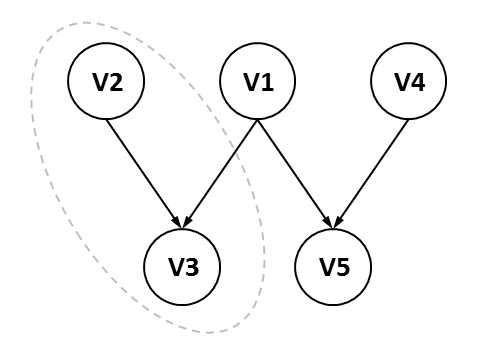
\includegraphics[width=1.6in]{figures/enum_mbpt1.png}}\hfill%
	\subcaptionbox{2b\label{enum_dup_b}}{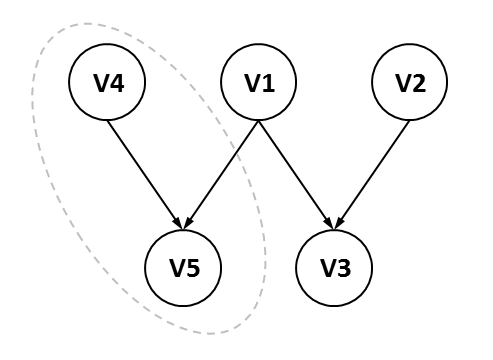
\includegraphics[width=1.6in]{figures/enum_mbpt2.png}}%
	\hspace*{\fill}%
	\caption{Example of two duplicated Markov blanket polytrees when enumerating.}
	\label{enum_duplicated}
\end{figure}

The total number of Markov blanket polytrees (MBPs) is dramatically reduced comparing with DAGs as shown in Table \ref{tb:nmbps}.

\begin{table}[]
\centering
\caption{The number of labelled DAGs and MBPs on $n \in [0, 7]$ nodes.}
\label{tb:nmbps}
\begin{tabular}{lll}
\hline
\# nodes & \# DAGs    & \# MBPTs \\ \hline
1        & 1          & 1        \\
2        & 3          & 2        \\
3        & 25         & 6        \\
4        & 543        & 23       \\
5        & 29281      & 104      \\
6        & 3781503    & 537      \\
7        & 1138779265 & 3100     \\ \hline
\end{tabular}
\end{table}

The message length for transmitting data using a MBP model is calculated as the natural log of the conditional probability
\begin{align*}
p(X_i|S) = \frac{p(X_i \mid \Pi_i^{T_i})\prod_{X_j \in S} p(X_j | \Pi_j^{T_i})}{\sum_{x_i=1}^{r_i}p(x_i \mid \Pi_i^{T_i})\prod_{X_j \in S} p(X_j | \Pi_j^{T_i})}
\end{align*}
is factorized into a product of each variable's probability conditioning on its parents set in a Markov blanket polytree $T_i$, which can be estimated from data using the adaptive code method. Hence, the total message length has the form 
\begin{align}
\label{eq:mmlmbp}
\begin{split}
I(\phi_i(S), D_{\phi_i}) = -\sum_{D_{\phi_i}} \biggl[
&\ln p(X_i\mid \Pi_i^{T_i}) + \sum_{X_j \in S} \ln p(X_j | \Pi_j^{T_i}) - \\
&\ln \sum_{x_i=1}^{r_i}p(x_i \mid \Pi_i^{T_i})\prod_{X_j \in S} p(X_j | \Pi_j^{T_i})
\biggr].
\end{split}
\end{align}
To calculate a weighted average score, we uniformly average the conditional probabilities $p(X_i\mid S)$ over all possible MBPs  $\mathcal{T}_i$ containing the same variables $\{X_i\} \cup MB_i$, then take the negative $\log$ of the expected probability. The uniform prior can be replaced by any reasonable prior over the possible Markov blanket polytrees.


\subsection{Pseudo-code of the MBMML algorithm}
This section presents the pseudo-code of two types of the MBMML algorithm that learns Markov blanket of a target variable using either a fixed local structure (i.e., CPT or NB) or an ensemble of random local structures (i.e., MBPs). Both algorithms use a greedy search starting with empty Markov blanket and iteratively adding the highest ranked candidate into the Markov blanket to reduce the total message length calculated by a MML metric (equation \ref{eq:mmlcpt} or \ref{eq:mmlnb}, or \ref{eq:mmlmbp}). Both algorithms stop and output a learned Markov blanket if no scores can be increased by adding more candidates. Algorithms \ref{alg:mbmmlf} and \ref{alg:mbmmlr} outline steps of the fixed and ensemble methods.

\begin{algorithm}[]
\caption{MB discovery using MBMML+CPT/NB}
\label{alg:mbmmlf}
\begin{algorithmic}[MBMML]
\Procedure{$MBMML$}{$X_i, X, D, \phi_i$}, where $X_i$ is the target variable, $X$ is the set of all variables, $D$ is a given dataset and $\phi_i$ is fixed to be either a CPT or  NB model.
    \State $S = X \setminus {X_i}$ \Comment{unchecked variables}
    \State $Z = \emptyset$ \Comment{learned MB}
    \State $L = I(\phi_i(\emptyset), D_{\phi_i})$  \Comment{empty model score}
    \While {$S \neq \emptyset$}
    		\State $X_k = \argmin_{X_j} I(\phi_i(Z \cup \{X_j\}), D_{\phi_i}), \forall X_j \in S$ \Comment{best candidate}
    		\State $L' = I(\phi_i(Z \cup \{X_k\}), D_{\phi_i})$ \Comment{current best score}
    		\If{$L' < L$} \Comment{admit when score reduces}
    			\State $Z = Z \cup \{X_k\}$
    			\State $S = S \setminus \{X_k\}$
    			\State $L = L'$ \Comment{update best score}
    		\Else
    			\State Stop 
			\EndIf
	\EndWhile
	\State Output $Z$
\EndProcedure
\end{algorithmic}
\end{algorithm}

% Insert the algorithm
\begin{algorithm}[]
\caption{MB discovery using MBMML+ENSEMBLE}
\label{alg:mbmmlr}
\begin{algorithmic}[MBMML]
\Procedure{$MBMML$}{$X_i, X, D, \phi_i, K$}, where $X_i$ is the target variable, $X$ is the set of all variables, $D$ is a given dataset, $\phi_i$ is a MBP model, $K$ is the number of randomly sampled MBPs. 
    \State $S = X \setminus {X_i}$ \Comment{unchecked variables}
    \State $Z = \emptyset$ \Comment{learned MB}
    \State $L = I(\phi_i(\emptyset), D_{\phi_i})$  \Comment{empty model score}
    \While {$S \neq \emptyset$}
    		\If{$f(|Z| + 1) \leq K$} \Comment{number of MBPs by equation \ref{eq:nmbps}}
    			\State $\mathcal{T}_i := \{\text{all MBPs over } Z \cup \{X_j\}\}$ \Comment{all MBPs}
    		\Else
    			\State $\mathcal{T}_i =  \{K \text{ random MBPs over } Z \cup \{X_j\}\}$ \Comment{randomly sampled MBPs}
    		\EndIf 
    		\State $X_k = \argmin_{X_j} E_{\mathcal{T}_i}(I(\phi_i(Z \cup \{X_j\}), D_{\phi_i})), \forall X_j \in S$ \Comment{best candidate}
    		\State $L' = E_{\mathcal{T}_i}(I(\phi_i(Z \cup \{X_k\}), D_{\phi_i}))$ \Comment{current best expected score}
    		\If{$L' < L$} \Comment{admit when score reduces}
    			\State $Z = Z \cup \{X_k\}$
    			\State $S = S \setminus \{X_k\}$
    			\State $L = L'$ \Comment{update best score}
    		\Else
    			\State Stop 
			\EndIf
	\EndWhile
	\State Output $Z$
\EndProcedure
\end{algorithmic}
\end{algorithm}

To ensure there is no conflict among the learned Markov blankets so that they can be used later for structure learning, we enforced outputs from both MBMML+CPT/N and MBMML+ENSEMBLE algorithms to satisfy the symmetry property as shown in section \ref{sec:mb}. There are two deterministic enforcements, by union or intersection between two learned Markov blankets. The process of the symmetry enforcement is shown in Algorithm \ref{alg:sym}. Throughout these experiments we applied the UNION enforcement to MBMML+CPT, because a CPT model's precision converges to $1$ as sample size increases. So its exponential increase in parameters is likely to result in more false negatives than false positives. The INTERSECTION enforcement was conducted on MBMML+NB, because a Na\"ive Bayes model intend to produce more false positives than a CPT model due to its lack of explanation power, but less false negatives because of its simplicity. It is not clear which enforcement is a better option for MBMML+ENSEMBLE, so we chose the UNION enforcement throughout the experiments. 

\begin{algorithm}[]
\caption{Symmetry enforcement}
\label{alg:sym}
\begin{algorithmic}[]
\Procedure{}{} Given the learned Markov blankets $\{MB_i\}, \forall X_i \in X$
\For{each $MB_i$}
	\For{each $X_j \in MB_i$}
		\If{$X_i \notin MB_j$}
			\If{UNION}
				\State $MB_j = MB_j \cup \{X_i\}$
			\Else{ INTERSECTION}
				\State $MB_i = MB_i \setminus \{X_j\}$
			\EndIf
		\EndIf
	\EndFor
\EndFor
	\State Output $\{MB_i\}$
\EndProcedure
\end{algorithmic}
\end{algorithm}


\section{Experiments on Markov blanket discovery}
In this section, we present some of the experimental results on comparing different Markov blanket learners. All three algorithms, MBMML+CPT, MBMML+NB, and MBMML+ENSEMBLE were tested against the following algorithms: 
\begin{itemize}
\item IAMB - a constraint-based algorithm that uses conditional independence test for candidate admission. It starts admitting variables that are dependent with the target conditioning on the current found Markov blanket. It is followed by a backward phase trying to delete any false positives.  
\item PCMB - a constraint-based algorithm that divides a learning into two sub-tasks. Firstly, it finds the direct neighbours of the target. It then finds the neighbours of each neighbour of the target, and prunes any false positives. This algorithm also relies on conditional independence test. 
\item SLL - a metric-based algorithm that uses dynamic programming and BDeu score. It is an exact algorithm that searches through the entire space of equivalence classes of local DAGs around a target, then reads off the optimal Markov blanket. Notice SLL does not just learn Markov blankets. It is for scaling up Bayesian network structure learning. 
\end{itemize}
We used the implementations of IAMB and PCMB provided by \cite{pena2007towards} and setted the significant level $\alpha=0.05$ for conditional independence test. We used SLL's source code provided by \cite{niinimaki2012local} and its default equivalent sample size $1$ for BDeu. SLL fallbacks to GES algorithm \cite{chickering2002learning} if it tends to find more than $20$ variables for a Markov blanket. The three MML methods assumed uniform parameter prior (i.e., symmetric Dirichlet with concentration parameter $\vec{\alpha} = <1>$). The MBMML+ENSEMBLE algorithm was setted to randomly sample $100$ Markov blanket polytrees from the entire space and uniformly averaged their message lengths. 
%The IPCMB algorithm has been experimentally justified to outperform IAMB and PCMB. And the IPCMB recently has been justified to be less superior than SLL and STMB \cite{gao2017efficient} on similar datasets. 

Section \ref{sec:exp_real} focuses on testing with real models (Table \ref{tab:exp_models})and standard datasets provided by \footnote{\url{http://www.dsl-lab.org/supplements/mmhc_paper/mmhc_index.html\#complete_data}}. The sample size varies in $500, 1000, 5000$ and each size comes with $10$ different datasets. These models are often used for testing Markov blanket and causal discovery learners.  Section \ref{sec:exp_artificial} extends the experiments to artificial Bayesian networks (\ref{tab:exp_models}) containing $30$ and $50$ variables respectively, and the same maximum fan-in and number of states for each variable. For each model specification, we randomly generate $5$ different Bayesian networks, each of which was then used to generate $5$ different datasets for every one of the sample sizes $100, 500, 2000, 5000$. 

The evaluation metrics used are precision, recall, and edit distance. The edit distance between a true Markov blanket and a learned Markov blanket is equal to the sum of false positives and false negatives. The average accuracy over all variables in one structure and all samples with the same size were reported with $95\%$ confidence intervals. Due to space limit, only selected models were discussed in the main text. The rest of the results are included in the appendix. 
\begin{table}
% table caption is above the table
\caption{Summary of tested Bayesian networks. 30-5-4-1 and 30-5-4-1 refer to artificial networks with 30 and 50 variables, maximum fan-in 5, maximum number of states 4, and uniform ($\vec{\alpha}=<1>$) parameter prior.}
\label{tab:exp_models}       
\begin{tabular}{llll}
\hline\noalign{\smallskip}
Network    & Number of odes & Max fan-in & Mean MB size  \\
\noalign{\smallskip}\hline\noalign{\smallskip}
CHILD      & 20    & 2  &  3 \\
INSURANCE & 27    & 3  &  5.19 \\
ALARM     & 37   & 4  & 3.51 \\  
BARLEY & 48 & 4 & 5.25 \\
HAILFINDER & 56 & 4 & 3.54 \\
30-5-4-1 & 30 & 5 & 8 \\
50-5-4-1 & 50 & 5 & 9.73 \\
\noalign{\smallskip}\hline
\end{tabular}
\end{table}


\subsection{Accuracy on real models}
\label{sec:exp_real}
Figures \ref{fg:child} and \ref{fg:barley} report the mean edit distance (with confidence intervals) of all algorithms on the CHILD and BARLEY networks. In both cases, IAMB has the lowest accuracy given any sample size. In most cases, the other algorithms show no statistically significant difference from each other, except PCMB and MML+ENSEMBLE are less robust under small samples. Both PCMB and SLL have shown a projection of faster convergence than MML methods and IAMB. Noticing that PCMB failed to run on the BARLEY network possibly due to an implementation error. The edit distance and precision and reacall on all five models are summarized in Table \ref{tb:all_ed} and Table \ref{tb:all_pre_rec} (in appendix) respectively. In general, on these real networks SLL has most of the winnings followed, MBMML+CPT, MBMML+NB, PCMB, MBMML+ENSEMBLE and IAMB. 
\begin{figure}[H]
  \centering
    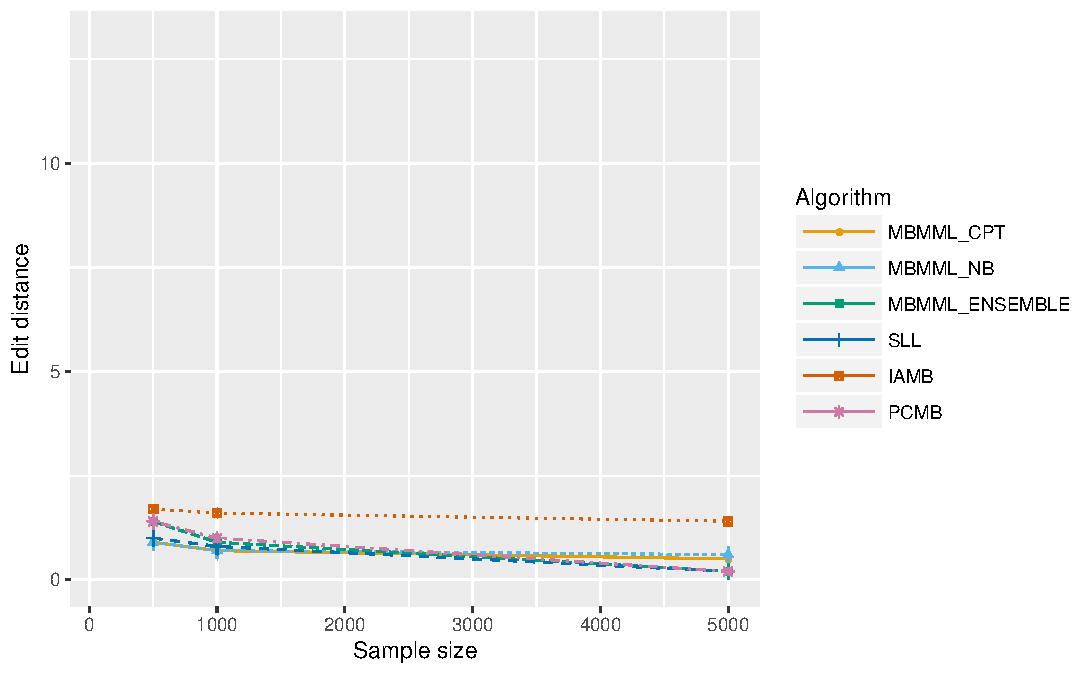
\includegraphics[scale=0.6]{figures/ed_vs_samplesize_child.pdf}
  \caption{Edit distance (with $95\%$ confidence intervals) v.s. sample size on CHILD network.}
  \label{fg:child}
\end{figure}

\begin{figure}[H]
  \centering
    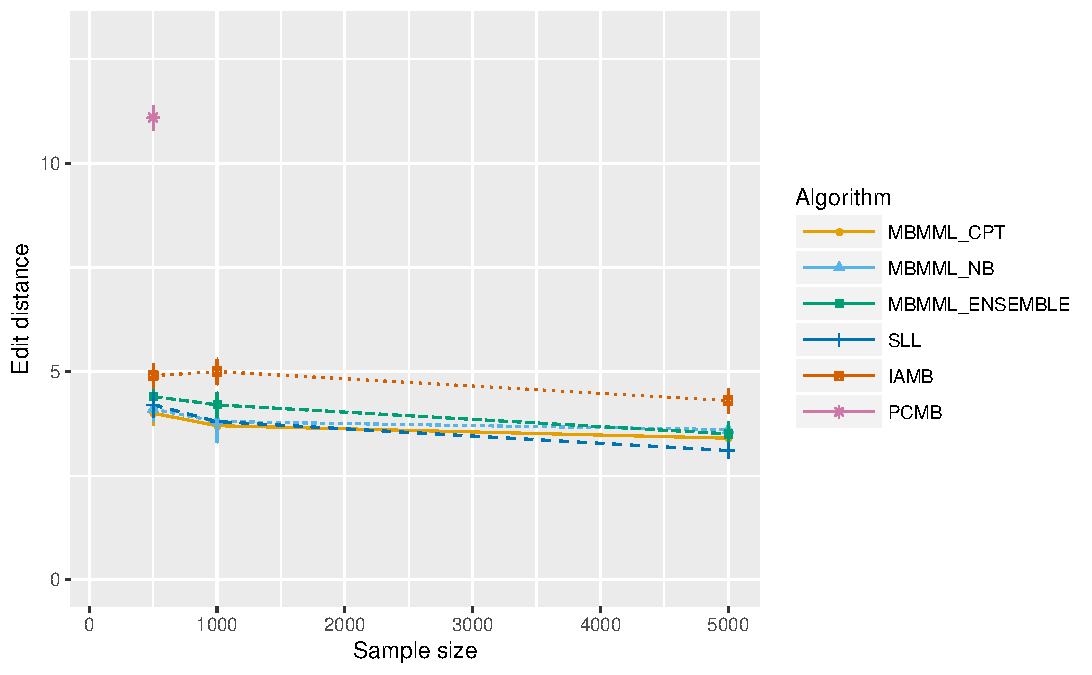
\includegraphics[scale=0.6]{figures/ed_vs_samplesize_barley.pdf}
  \caption{Edit distance (with $95\%$ confidence intervals) v.s. sample size on BARLEY network. PCMB failed under 1000 and 5000 samples possibly due to an implementation error.}
  \label{fg:barley}
\end{figure}

\subsection{Accuracy on artificial models} 
\label{sec:exp_artificial}
To test all metods on different problems over a number of random networks, we generated 5 different Bayesian networks for each pre-specified model specification. These networks are moderate in the number of nodes, and slightly larger comparing with the real networks used before in maximum fan-in and average Markov blanket size. Their parameters were sampled from uniform distribution which matches the parameter prior used in the multi-state MML metric. This may be an advantage of the MML methods for these particular problems, but it is less risky when nothing is known about the models. Later in this section, it has been shown briefly that this uninformative prior could produce similar accuracy as using the true prior.  

Figure \ref{fg:30} and \ref{fg:50} have shown how the tested methods reacted to different sample sizes on artificial networks with specification 30-5-4-1 and 50-5-4-1. The MBMML+NB and IAMB algorithms started well under extreme small samples but could not converge given more samples. This is likely to be caused by the lack of representation power of Naive Bayes models and the unsoundness of IAMB. The MBMML+CPT and MBMML+ENSEMBLE algorithms have shown competitive performances under both small and large samples, and superior low edit distance for moderate samples, but both methods converged slower than PCMB and SLL towards 5000 samples. The main issue is believed to be the exponential number of parameters in both CPT and MBPT models. Both PCMB and SLL converged faster than the others like in the real model cases. The former, however, had the worst accuracy under 100 samples whilst the later are  almost no difference from the others. 
\begin{figure}[H]
  \centering
    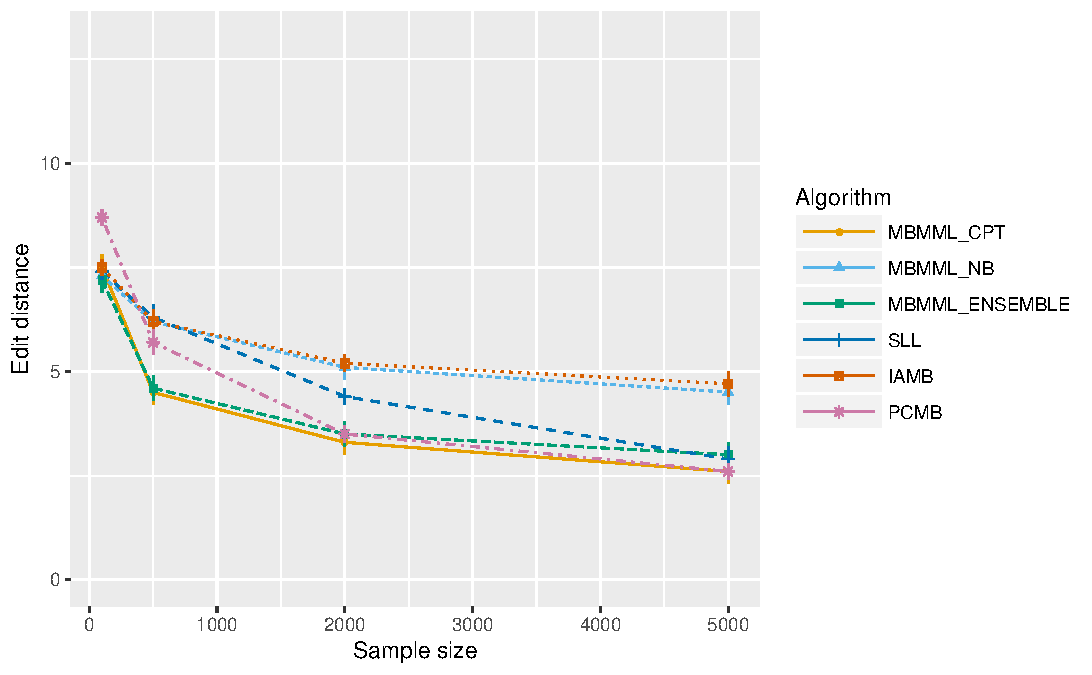
\includegraphics[scale=0.6]{figures/ed_vs_samplesize_30_5_4_1.pdf}
  \caption{Edit distance (with $95\%$ confidence intervals) v.s. sample size on artificial Bayesian networks (30-5-4-1) containing 30 variables, maximum 5 parents and maximum 4 states for each variable.}
  \label{fg:30}
\end{figure}

\begin{figure}[H]
  \centering
    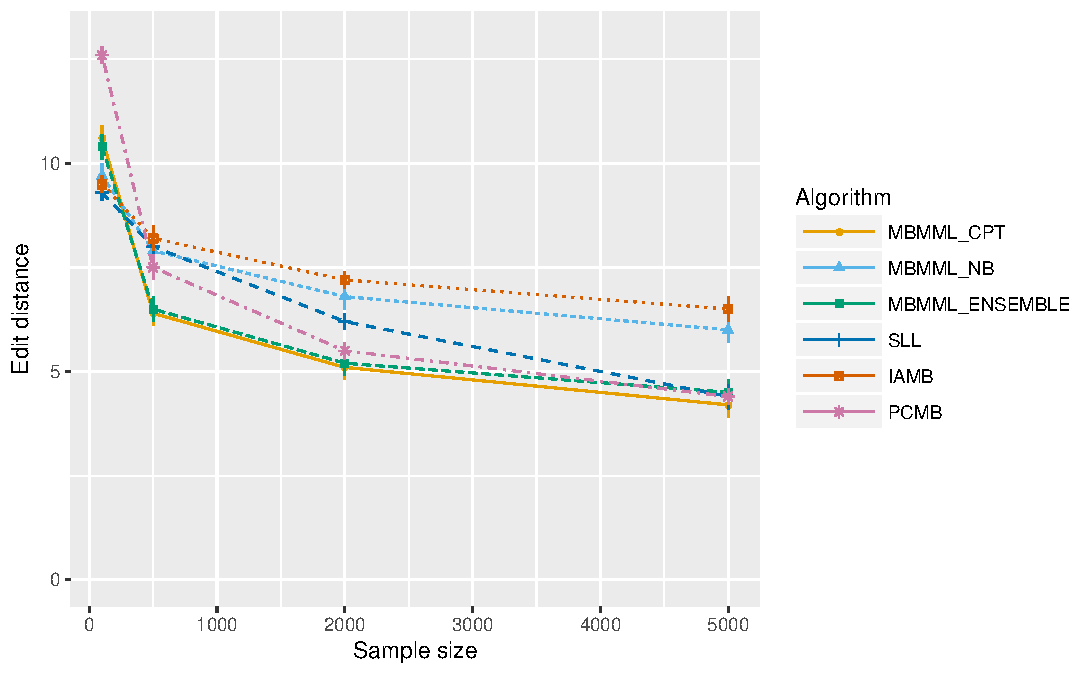
\includegraphics[scale=0.6]{figures/ed_vs_samplesize_50_5_4_1.pdf}
  \caption{Edit distance (with $95\%$ confidence intervals) v.s. sample size on artificial Bayesian networks (50-5-4-1) containing 50 variables, maximum 5 parents and maximum 4 states for each variable.}
  \label{fg:50}
\end{figure}

So far, we have investigated the overall performance of Markov blanket learners given some networks. Now, we group together problems having similar complexity and look for the trend when increasing Markov blanket size. Figure \ref{fg:ed_mb_50_500} and \ref{fg:ed_mb_50_5000} are edit distances of all methods for different Markov blanket size given 500 and 5000 samples respectively. The rest of the results are contained in the appendix.  

\begin{figure}[H]
  \centering
    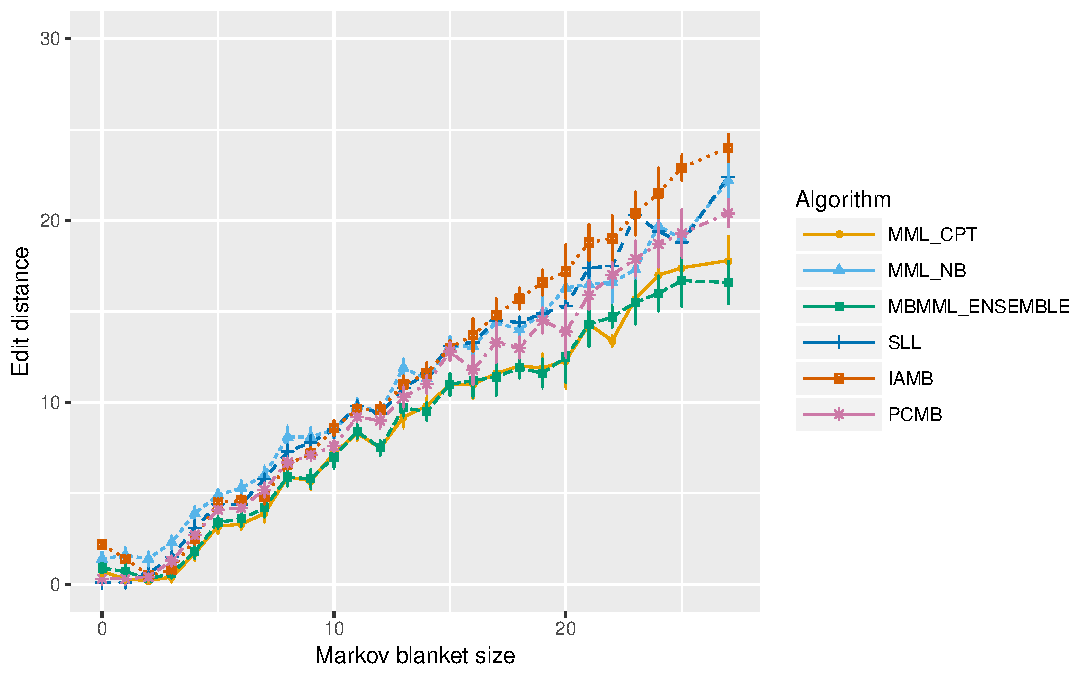
\includegraphics[scale=0.6]{figures/ed_vs_mbsize_50_5_4_1_500.pdf}
  \caption{Edit distance against Markov blanket size on 50-5-4-1 models with 500 samples.}
  \label{fg:ed_mb_50_500}
\end{figure} 
Given 500 samples (Figure \ref{fg:ed_mb_50_500}) for 50 variables networks, PCMB and SLL did well by identifying unconnected variables, whilst the others more or less had some false positives. As Markov blanket size was increased, the MBMML+CPT and MBMML+ENSEMBLE algorithms produced the fewest false findings all the way up to the maximum Markov blankets. It is worth noticing that for Markov blankets over 20 variables, it is GES's performance instead of SLL. On averaged, MBMML+CPT and MBMML+ENSEMBLE have the lowest edit distance which is consistent with the ranking in Figure \ref{fg:50} for 500 samples. 

\begin{figure}[H]
  \centering
    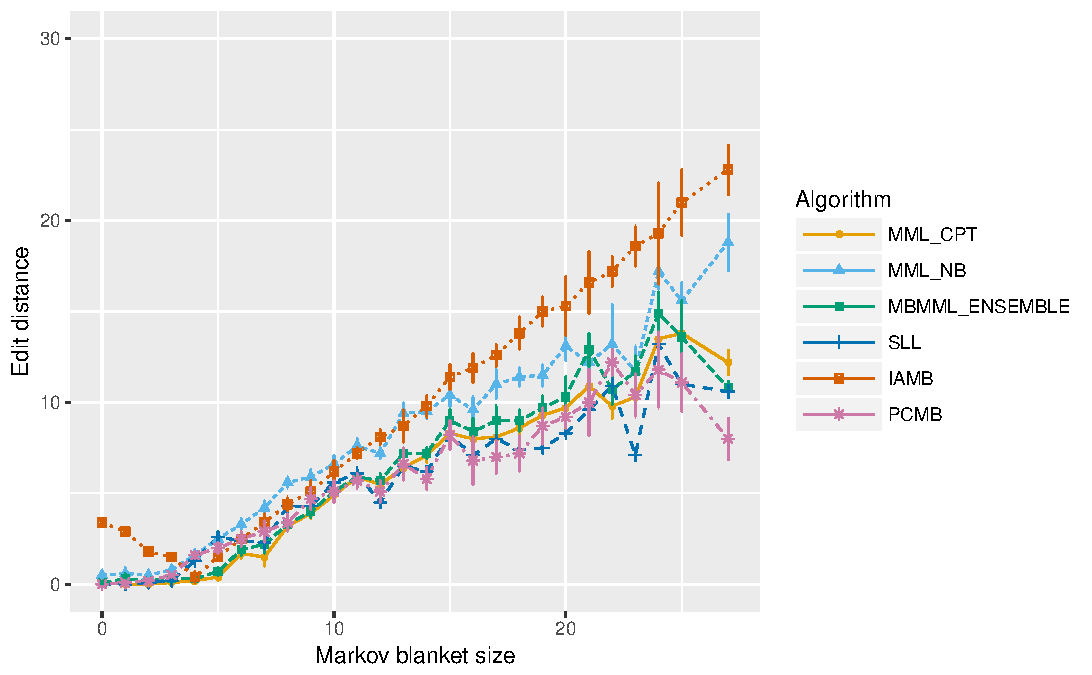
\includegraphics[scale=0.6]{figures/ed_vs_mbsize_50_5_4_1_5000.pdf}
  \caption{Edit distance against Markov blanket size on 50-5-4-1 models with 5000 samples.}
  \label{fg:ed_mb_50_5000}
\end{figure}
Given 5000 samples (Figure \ref{fg:ed_mb_50_5000}), most methods did well for Markov blanket size smaller than 4 except IAMB, who had a wired U-shape where the bottom is at 4 variables. MBMML+CPT and MBMML+ENSEMBLE kept the lowest edit distance for medium Markov blankets, but were unable to keep it low as the learning problems became more complex so being outperformed occasionally by PCMB and SLL. In summary, the two MML methods except MBMML+NB have lowest error rate for medium-sized learning problems given moderate samples. 

There may be a concern that if the generating models used a non-uniform prior, the MML methods could produce different results. In principle, if the true prior is not uniform, using uniform prior would give no better results than uing the true prior. In practice, however, it is also depends on the quality and size of samples. To show the impact of using uninformative prior, MBMML+CPT was given both the true prior and uniform prior then tested on a 30-5-4-1 network whose parameters were sampled from a symmetric Dirichlet distribution with different concentration parameter $\alpha \in \{0.1, 0.4, 0.7, 1, 10, 40, 70, 100\}$. The experiments were completed for 500 and 5000 samples. 

Figure \ref{fg:wrong_prior_500} and \ref{fg:wrong_prior_5000} have shown insiginificant difference between the use of true prior and uniform prior for the case when the concentration parameters $\alpha \le 1$. This is because adding small $\alpha$ values to parameter estimations almost do not matter when there exists at last some data for each parameter. When $\alpha > 1$, uniform prior produced slightly less edit distance than the true prior. By looking into the number of learned Markov blanket size, we notice that as $\alpha$ increases the learned Markov blankets also increase in size. It is believed that this is caused by the same reason as the sensitivity of BDeu as shown by \cite{silander2007sensitivity}. The MML metric for CPT model with symmetric Dirichlet prior is similar as the BDeu metric, except the former includes costs for stating estimated parameters and used uniform Dirichlet prior over all model parameters whilst the later does not state parameters and only used uniform Dirichlet prior over parameters of each node. But both metrics penalise model complexity using a function of $\alpha$, which decreases as $\alpha$ increases. Hence, under large $\alpha$ the MML methods discovered larger Markov blankets which could contain a large propotion of false positives especially under small samples. This is also why when using 5000 samples, the true prior produced similar edit distance as uniform prior.

\begin{figure}[H]
  \centering
    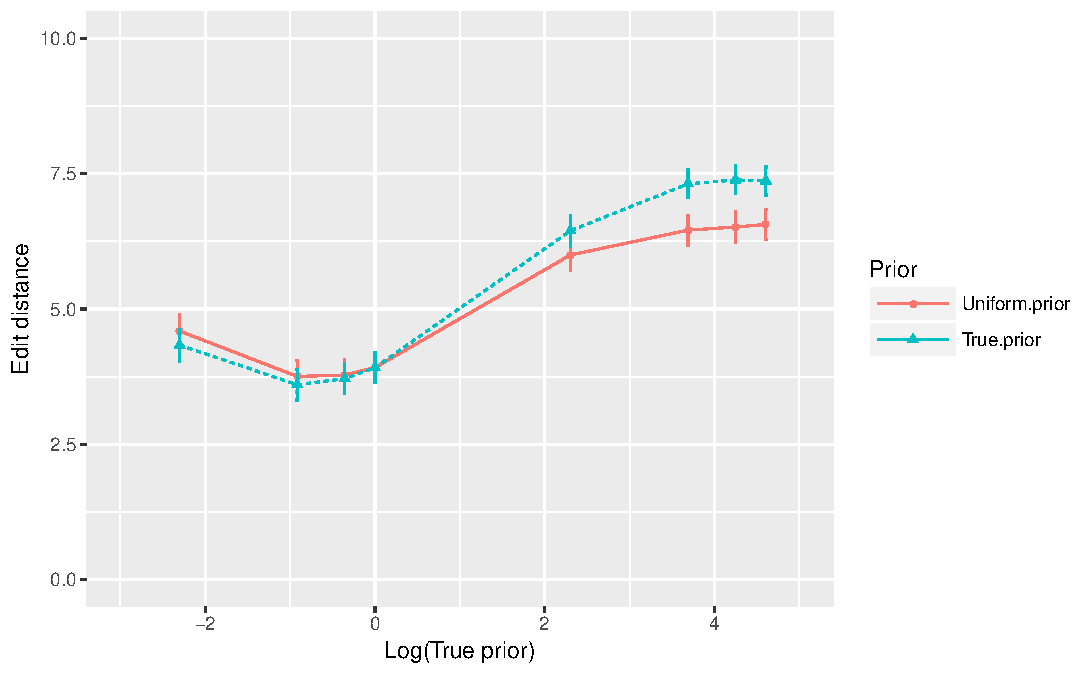
\includegraphics[scale=0.6]{figures/ed_vs_trueprior_30_5_4_alpha_134445_500.pdf}
  \caption{MBMML+CPT's edit distances using the true prior and uniform prior on a 30-5-4-1 model with 500 samples. The X-axis is the natural log scale of the true symmetric Dirichlet concentration parameter $\alpha = \{0.1, 0.4, 0.7, 1, 10, 40, 70, 100\}$.}
  \label{fg:wrong_prior_500}
\end{figure}

\begin{figure}[H]
  \centering
    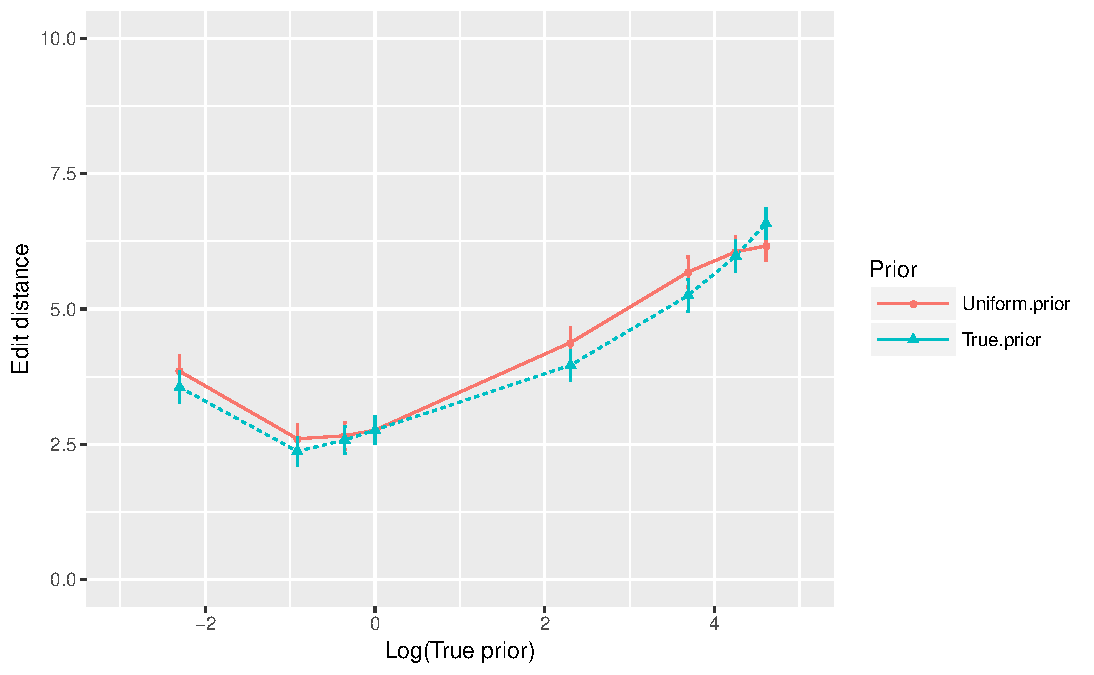
\includegraphics[scale=0.6]{figures/ed_vs_trueprior_30_5_4_alpha_134445_5000.pdf}
  \caption{MBMML+CPT's edit distances using the true prior and uniform prior on a 30-5-4-1 model with 5000 samples. The X-axis is the natural log scale of the true symmetric Dirichlet concentration parameter $\alpha = \{0.1, 0.4, 0.7, 1, 10, 40, 70, 100\}$.}
  \label{fg:wrong_prior_5000}
\end{figure}

\subsection{Algorithm complexity}
Table \ref{tb:bigo} orders all algorithms by ascending computational complexity. The while loop in Algorithm \ref{alg:mbmmlf} runs at most $n-1$ times. Each time it runs through all unchecked nodes to find the best candidate according to a MML metric. For a CPT model, there could be at most $n-1$ parents in which case the multi-state MML is summed over all $2^{n-1}$ parents instantiations. So the computational complexity of the MBMML+CPT algorithm is $O(n2^{n-1})$. For a NB model, the worst case is when all $n-1$ nodes are children of the target, which is linear in $n$ within the \textit{WHILE} loop, so gives a complexity $O(n^2)$. The worst case of MBMML+RANDOM is when a CPT model appears in the sampled Markov blanket polytrees. In general, a random model is slower than a CPT by a constant factor, which is determined by the number of sampled local structures. But it has the same complexity as a CPT model. For PCMB, the total time required is dominated by the process of finding the direct neighbours of the target. This process tries to find a subset of the neighbour set, conditioning on which the target is independent with a candidate. And such a process runs through all variables to ensure the symmetry property. Hence, its complexity in the worst case is $O(n^2 2^{n-1})$. The total time required by IAMB and SLL were published in the associated papers. 
\begin{table}[]
\centering
\caption{Algorithm's computational complexity in big O notation.}
\label{tb:bigo}
\begin{tabular}{ll}
\hline
Algorithm    & Big O notation \\ \hline
IAMB      & $O(n^2)$      \\
MBMML+NB          &    $O(n^2)$    \\
MBMML+CPT          &   $O(n2^{n-1})$      \\
MBMML+RANDOM         & $O(n2^{n-1})$        \\
PCMB & $O(n^2 2^{n-1})$     \\
SLL        & $O(n^4 2^n)$       \\ \hline 
\end{tabular}
\end{table}


\section{Conclusion}
\label{sec:disc}

This paper presented three MML methods for learning Markov blankets of variables. The three methods are all built based on the multi-state MML metric, but associated with different models that are CPT, Naive Bayes and an ensemble of random Markov blanket polytree models. The MBMML+CPT algorithm was proven to be correct under infinite samples, though may not be data efficient for large Markov blankets due to exponential number of parameters. The MBMML+NB algorithm was developed to overcome the problem of exponential model complexity by sacrificing the the modelling of variable interactions. Both methods have no tendency of learning the subgraphs within Markov blankets, although certain model structures are assumed during learning. Realizing it is restricted to consider only a particular model structure for learning Markov blankets, we generalised to the MBMML+ENSEMBLE algorithm that assesses the validity of a variable being in a Markov blanket under random polytrees within Markov blankets. The search algorithms used are greedy search but can be replaced with any heuristics or probabilistic searches. The three MML algorithms were tested against several other Markov blanket algorithms on both real and artificial Bayesian networks given different sample sizes. In general, MBMML+CPT and MBMML+ENSEMBLE show superior results given moderate samples than the others. In particular, they had the lowest edit distance when learning medium-sized Markov blankets. The method with Naive Bayes model occationally appeared to be competitive for very small samples but could not converge given more samples. Comparing with the approximate algorithm PCMB, the two MML methods have advantages in both accuracy and efficiency, especially under small and medium samples. Comparing with the exact learning algorithm SLL, they are competitive in accuracy and faster in computational complexity by a factor of $n^3$. 

%In this paper, we proposed the \mbptmml algorithm that uses local-to-global paradigm to scale up general causal discovery algorithm to larger models with encouraging accuracy. \mbptmml's local step focuses on learning a local structure named MBPTs, the total number of which has been proved to be sub-exponential comparing with DAGs. Empirical evaluations against local-to-global and general causal learners suggested that \mbptmml is a competitive algorithm in most cases with some exceptions perhaps because of inappropriate prior used in MML. Although the test on execution time is not rigorous enough, meaning there are other factors such as machine specification, proper analysis of speed different between programming languages etc., that could have been controlled. It provides an estimation of \mbptmml's efficiency comparing with other types of learns, especially when comparing with those that adopted dynamic programming for optimal output. Although the current results are promising, \mbptmml has rooms to be improved. We have shown that inaccurate local variable and structure learnings can easily deviate a LGL learner from converging to generating models. To overcome this problem, we will consider several different roles of a new node in a MBPT structure to obtain an averaged prediction to a target. We believe this could avoid having a full CPT and hence further improve the recall of the current \mmlcpt process. The current version of \mbptmml extends onto global structures in a deterministic way, a potential improvement is to consider this step probabilistically such as giving these local adjacencies to CaMML as prior, hence reduce CaMML's sampling space so that models with higher posterior probability will be more accurately estimated in CaMML's MCMC step. By doing so, CaMML will be enabled to learn larger models that the current CaMML failed to do such as in CHILD5 and ALARM5. 


\newpage
\section{appendix}

\begin{table}[]
\centering
\caption{Summary of edit distance (with $95\%$ confidence intervals) of all Markov blanket discovery algorithms on both real and artificial Bayesian networks. The best results are highlighted in grey. In real networks, SLL wins most of the times followed by MBMML+CPT, MBMML+NB, PCMB, MMLL+ENSEMBLE, IAMB. PCMB failed to learn on BARLEY networks under 1000 and 5000 samples possibly due to an implementation error. In artificial networks, MBMML+CPT and MBMML+ENSEMBLE win most of the times followed by SLL, PCMB, MBMML+NB, IAMB.}
\label{tb:all_ed}
\begin{tabular}{llllllll}
\hline
Network    & SAMPLES &  \begin{tabular}[c]{@{}l@{}}$MBMML$\\ $+CPT$\end{tabular} &  \begin{tabular}[c]{@{}l@{}}$MBMML$\\ $+NB$\end{tabular} & \begin{tabular}[c]{@{}l@{}}$MBMML$\\ $+ENSEMBLE$\end{tabular} & IAMB     & PCMB     & SLL      \\ \hline
CHILD      & 500     & \cellcolor{lightgray}0.9+-0.2      & \cellcolor{lightgray}0.9+-0.2     & 1.4+-0.2  & 1.7+-0.2 & 1.4+-0.2 & \cellcolor{lightgray}1+-0.2   \\
           & 1000    & \cellcolor{lightgray}0.7+-0.1      & \cellcolor{lightgray}0.7+-0.2     & \cellcolor{lightgray}0.9+-0.2  & 1.6+-0.2 & \cellcolor{lightgray}1+-0.2   & \cellcolor{lightgray}0.8+-0.1 \\
           & 5000    & 0.5+-0.1      & 0.6+-0.1     & \cellcolor{lightgray}0.2+-0.1  & 1.4+-0.2 & \cellcolor{lightgray}0.2+-0.1 & \cellcolor{lightgray}0.2+-0.1 \\ \hline
INSURANCE  & 500     & \cellcolor{lightgray}3.3+-0.2      & \cellcolor{lightgray}3.5+-0.2     & 3.7+-0.3  & \cellcolor{lightgray}3.6+-0.3 & \cellcolor{lightgray}3.4+-0.2 & \cellcolor{lightgray}3.1+-0.2 \\
           & 1000    & \cellcolor{lightgray}2.9+-0.2      & 3.3+-0.2     & \cellcolor{lightgray}3.1+-0.3  & 3.7+-0.3 & \cellcolor{lightgray}3+-0.2   & \cellcolor{lightgray}2.7+-0.2 \\
           & 5000    & \cellcolor{lightgray}2.1+-0.2      & 2.8+-0.2     & 2.4+-0.2  & 2.8+-0.2 & \cellcolor{lightgray}1.8+-0.2 & \cellcolor{lightgray}2+-0.2   \\ \hline
ALARM      & 500     & 1.4+-0.1      & 2.1+-0.2     & 2.3+-0.2  & 2.2+-0.2 & 1.7+-0.2 & \cellcolor{lightgray}0.8+-0.1 \\
           & 1000    & 1+-0.1        & 1.8+-0.2     & 1.9+-0.2  & 2+-0.2   & 1.1+-0.1 & \cellcolor{lightgray}0.6+-0.1 \\
           & 5000    & 0.5+-0.1      & 1.5+-0.2     & 1.5+-0.1  & 1.5+-0.2 & \cellcolor{lightgray}0.2+-0.1 & \cellcolor{lightgray}0.2+-0   \\ \hline
BARLEY     & 500     & \cellcolor{lightgray}4+-0.3        & \cellcolor{lightgray}4.1+-0.3     & \cellcolor{lightgray}4.4+-0.3  & 4.9+-0.3 & 11.1+-0.5 & \cellcolor{lightgray}4.2+-0.2 \\
           & 1000    & \cellcolor{lightgray}3.7+-0.3      & \cellcolor{lightgray}3.8+-0.3     & \cellcolor{lightgray}4.2+-0.3  & 5+-0.3 & NA & \cellcolor{lightgray}3.8+-0.2 \\
           & 5000    & \cellcolor{lightgray}3.4+-0.3      & \cellcolor{lightgray}3.6+-0.3     & \cellcolor{lightgray}3.5+-0.3  & 4.3+-0.3 & NA & \cellcolor{lightgray}3.1+-0.2 \\ \hline
HAILFINDER & 500     & \cellcolor{lightgray}4.4+-0.3      & \cellcolor{lightgray}4.3+-0.2      & 5.2+-0.3  & \cellcolor{lightgray}4.2+-0.2 & 7.6+-0.5 & \cellcolor{lightgray}4.3+-0.3 \\
           & 1000    & \cellcolor{lightgray}4.4+-0.3      & \cellcolor{lightgray}4.3+-0.2     & 5+-0.3    & \cellcolor{lightgray}4.5+-0.2 & 6.7+-0.4 & \cellcolor{lightgray}4.1+-0.3 \\
           & 5000    & \cellcolor{lightgray}4.3+-0.3      & \cellcolor{lightgray}4.3+-0.2       & 5.1+-0.3  & 5.1+-0.2 & \cellcolor{lightgray}3.9+-0.2 & \cellcolor{lightgray}4+-0.3  \\ \hline
30-5-4-1   & 100     & \cellcolor{lightgray}7.5+-0.3      & \cellcolor{lightgray}7.3+-0.3     & \cellcolor{lightgray}7.2+-0.3  & \cellcolor{lightgray}7.5+-0.3 & 8.7+-0.3 & \cellcolor{lightgray}7.4+-0.3 \\
		   & 500     & \cellcolor{lightgray}4.5+-0.3      & 6.3+-0.3     & \cellcolor{lightgray}4.6+-0.3  & 6.2+-0.3 & 5.7+-0.3 & 6.3+-0.3 \\
           & 2000    & \cellcolor{lightgray}3.3+-0.2      & 5.1+-0.3     & \cellcolor{lightgray}3.5+-0.2  & 5.2+-0.3 & \cellcolor{lightgray}3.5+-0.2 & 4.4+-0.3 \\
           & 5000    & \cellcolor{lightgray}2.6+-0.2      & 4.5+-0.2     & \cellcolor{lightgray}3+-0.2    & 4.7+-0.3 & \cellcolor{lightgray}2.6+-0.2 & \cellcolor{lightgray}2.9+-0.2 \\ \hline
50-5-4-1   & 100     & 10.66+-0.3      & \cellcolor{lightgray}9.7+-0.3     & 10.4+-0.3  & \cellcolor{lightgray}9.5+-0.3 & 12.6+-0.3 & \cellcolor{lightgray}9.3+-0.3   \\
		   & 500     & \cellcolor{lightgray}4.5+-0.3      & 6.3+-0.3     & \cellcolor{lightgray}4.6+-0.3  & 6.2+-0.3 & 5.7+-0.3 & 6.3+-0.3 \\
           & 2000    & \cellcolor{lightgray}5.1+-0.2      & 6.9+-0.3     & \cellcolor{lightgray}5.2+-0.2  & 7.2+-0.3 & \cellcolor{lightgray}5.5+-0.2 & 6.2+-0.3 \\
           & 5000    & \cellcolor{lightgray}4.2+-0.2      & 6.1+-0.2     & \cellcolor{lightgray}4.5+-0.2  & 6.5+-0.3 & \cellcolor{lightgray}4.4+-0.2 & \cellcolor{lightgray}4.4+-0.2 \\ \hline
\end{tabular}
\end{table}

\begin{landscape}
%\begin{table}[]
\begin{center}
\scalebox{0.7}{
\label{tb:all_pre_rec}
\begin{tabular}{llllllllllllll}
\hline
Network    & SAMPLES & \multicolumn{2}{c}{MBMML+CPT}                          & \multicolumn{2}{c}{MBMML+NB}                           & \multicolumn{2}{c}{MBMML+RANDOM}                              & \multicolumn{2}{c}{IAMB}                                   & \multicolumn{2}{c}{PCMB}                                   & \multicolumn{2}{c}{SLL}                                    \\
           &         & \multicolumn{1}{c}{Precision} & \multicolumn{1}{c}{Recall} & \multicolumn{1}{c}{Precision} & \multicolumn{1}{c}{Recall} & \multicolumn{1}{c}{Precision} & \multicolumn{1}{c}{Recall} & \multicolumn{1}{c}{Precision} & \multicolumn{1}{c}{Recall} & \multicolumn{1}{c}{Precision} & \multicolumn{1}{c}{Recall} & \multicolumn{1}{c}{Precision} & \multicolumn{1}{c}{Recall} \\ \hline
CHILD      & 500     & 0.94+-0.03                    & 0.8+-0.04                  & 0.94+-0.03                    & 0.82+-0.04                 & 0.76+-0.04                    & 0.89+-0.03                 & 0.83+-0.04                    & 0.73+-0.04                 & 0.83+-0.04                    & 0.81+-0.04                 & 0.94+-0.03                    & 0.78+-0.04                 \\
           & 1000    & 0.98+-0.02                    & 0.88+-0.03                 & 0.97+-0.02                    & 0.86+-0.03                 & 0.82+-0.03                    & 0.96+-0.01                 & 0.81+-0.03                    & 0.81+-0.03                 & 0.91+-0.03                    & 0.84+-0.03                 & 0.97+-0.02                    & 0.84+-0.03                 \\
           & 5000    & 1+-0.01                       & 0.91+-0.02                 & 1+-0.01                       & 0.89+-0.02                 & 0.95+-0.02                    & 1+-0                       & 0.77+-0.04                    & 0.91+-0.02                 & 0.98+-0.01                    & 0.99+-0.01                 & 1+-0                          & 0.97+-0.01                 \\ \hline
INSURANCE  & 500     & 0.82+-0.04                    & 0.48+-0.03                 & 0.8+-0.04                     & 0.42+-0.03                 & 0.7+-0.04                     & 0.6+-0.03                  & 0.86+-0.03                    & 0.44+-0.03                 & 0.75+-0.04                    & 0.52+-0.03                 & 0.83+-0.04                    & 0.51+-0.04                 \\
           & 1000    & 0.86+-0.03                    & 0.54+-0.03                 & 0.85+-0.04                    & 0.45+-0.03                 & 0.76+-0.03                    & 0.65+-0.03                 & 0.78+-0.03                    & 0.5+-0.03                  & 0.79+-0.04                    & 0.56+-0.03                 & 0.88+-0.03                    & 0.58+-0.03                 \\
           & 5000    & 0.95+-0.01                    & 0.68+-0.03                 & 0.93+-0.02                    & 0.57+-0.03                 & 0.82+-0.03                    & 0.76+-0.03                 & 0.86+-0.02                    & 0.66+-0.03                 & 0.93+-0.03                    & 0.71+-0.03                 & 0.98+-0.01                    & 0.69+-0.03                 \\ \hline
ALARM      & 500     & 0.85+-0.03                    & 0.77+-0.03                 & 0.79+-0.03                    & 0.67+-0.03                 & 0.66+-0.03                    & 0.87+-0.02                 & 0.81+-0.03                    & 0.65+-0.03                 & 0.84+-0.03                    & 0.71+-0.03                 & 0.92+-0.02                    & 0.89+-0.02                 \\
           & 1000    & 0.9+-0.02                     & 0.82+-0.03                 & 0.86+-0.02                    & 0.68+-0.03                 & 0.69+-0.03                    & 0.92+-0.02                 & 0.81+-0.02                    & 0.75+-0.03                 & 0.9+-0.02                     & 0.81+-0.03                 & 0.94+-0.01                    & 0.94+-0.01                 \\
           & 5000    & 0.97+-0.01                    & 0.93+-0.02                 & 0.95+-0.02                    & 0.7+-0.03                  & 0.75+-0.02                    & 0.95+-0.01                 & 0.79+-0.02                    & 0.89+-0.02                 & 1+-0                          & 0.96+-0.01                 & 0.98+-0.01                    & 0.98+-0.01                 \\ \hline
BARLEY     & 500     & 0.74+-0.03                    & 0.37+-0.03                 & 0.74+-0.03                    & 0.35+-0.02                 & 0.66+-0.03                    & 0.51+-0.03                 & 0.7+-0.04                            & 0.17+-0.01                         & 0.25+-0.01                            & 0.59+-0.03                         & 0.63+-0.04                    & 0.25+-0.02                 \\
           & 1000    & 0.79+-0.03                    & 0.42+-0.03                 & 0.79+-0.03                    & 0.37+-0.02                 & 0.68+-0.03                    & 0.57+-0.03                 & 0.63+-0.04                            & 0.19+-0.02                         & NA                            & NA                         & 0.72+-0.04                    & 0.35+-0.03                 \\
           & 5000    & 0.8+-0.03                     & 0.52+-0.03                 & 0.81+-0.03                    & 0.47+-0.02                 & 0.72+-0.03                    & 0.7+-0.03                  & 0.73+-0.03                            & 0.36+-0.03                         & NA                            & NA                         & 0.85+-0.03                    & 0.5+-0.03                  \\ \hline
HAILFINDER & 500     & 0.3+-0.03                     & 0.18+-0.02                 & 0.25+-0.03                    & 0.12+-0.01                 & 0.27+-0.03                    & 0.2+-0.02                  & 0.31+-0.03                            & 0.17+-0.02                         & 0.28+-0.03                            & 0.19+-0.02                         & 0.28+-0.03                    & 0.14+-0.02                 \\
           & 1000    & 0.31+-0.03                    & 0.22+-0.02                 & 0.26+-0.03                    & 0.12+-0.01                 & 0.29+-0.03                    & 0.24+-0.02                 & 0.29+-0.03                            & 0.19+-0.02                         & 0.32+-0.03                            & 0.21+-0.02                         & 0.3+-0.03                     & 0.18+-0.02                 \\
           & 5000    & 0.34+-0.03                    & 0.26+-0.02                 & 0.26+-0.03                    & 0.14+-0.02                 & 0.3+-0.03                     & 0.27+-0.03                 & 0.24+-0.02                            & 0.23+-0.02                         & 0.32+-0.03                            & 0.21+-0.02                         & 0.34+-0.03                    & 0.22+-0.02                 \\ \hline
30-5-4-1   & 100     & 0.56+-0.02                    & 0.36+-0.02                 & 0.6+-0.03                     & 0.23+-0.02                 & 0.58+-0.02                    & 0.36+-0.02                 & 0.69+-0.03                    & 0.16+-0.01                 & 0.43+-0.02                    & 0.37+-0.02                 & 0.5+-0.03                     & 0.17+-0.02                 \\
           & 500     & 0.91+-0.02                    & 0.56+-0.02                 & 0.86+-0.02                    & 0.35+-0.02                 & 0.86+-0.02                    & 0.56+-0.02                 & 0.84+-0.02                    & 0.37+-0.02                 & 0.87+-0.02                    & 0.41+-0.02                 & 0.79+-0.03                    & 0.3+-0.02                  \\
           & 2000    & 0.97+-0.01                    & 0.68+-0.02                 & 0.94+-0.01                    & 0.48+-0.02                 & 0.94+-0.01                    & 0.68+-0.02                 & 0.89+-0.02                    & 0.51+-0.02                 & 0.93+-0.01                    & 0.69+-0.02                 & 0.94+-0.02                    & 0.54+-0.02                 \\
           & 5000    & 0.99+-0                       & 0.76+-0.02                 & 0.96+-0.01                    & 0.57+-0.02                 & 0.96+-0.01                    & 0.73+-0.02                 & 0.87+-0.02                    & 0.58+-0.02                 & 0.91+-0.01                    & 0.82+-0.01                 & 0.98+-0.01                    & 0.7+-0.02                  \\ \hline
50-5-4-1   & 100     & 0.44+-0.02                    & 0.28+-0.01                 & 0.47+-0.02                    & 0.19+-0.01                 & 0.42+-0.02                    & 0.27+-0.01                 & 0.61+-0.02                    & 0.12+-0.01                 & 0.31+-0.01                    & 0.31+-0.01                 & 0.45+-0.03                    & 0.12+-0.01                 \\
           & 500     & 0.85+-0.02                    & 0.46+-0.02                 & 0.77+-0.02                    & 0.29+-0.02                 & 0.8+-0.02                     & 0.46+-0.02                 & 0.79+-0.02                    & 0.3+-0.02                  & 0.81+-0.02                    & 0.33+-0.02                 & 0.74+-0.02                    & 0.26+-0.02                 \\
           & 2000    & 0.97+-0.01                    & 0.59+-0.02                 & 0.91+-0.01                    & 0.4+-0.02                  & 0.92+-0.01                    & 0.6+-0.02                  & 0.85+-0.02                    & 0.43+-0.02                 & 0.9+-0.01                     & 0.54+-0.02                 & 0.9+-0.02                     & 0.44+-0.02                 \\
           & 5000    & 0.99+-0                       & 0.68+-0.01                 & 0.97+-0.01                    & 0.49+-0.02                 & 0.97+-0.01                    & 0.67+-0.01                 & 0.87+-0.01                    & 0.51+-0.02                 & 0.91+-0.01                    & 0.68+-0.01                 & 0.96+-0.01                    & 0.6+-0.02                  \\ \hline
\end{tabular}}
\end{center}
%\end{table}
\end{landscape}

\begin{figure}[H]
  \centering
    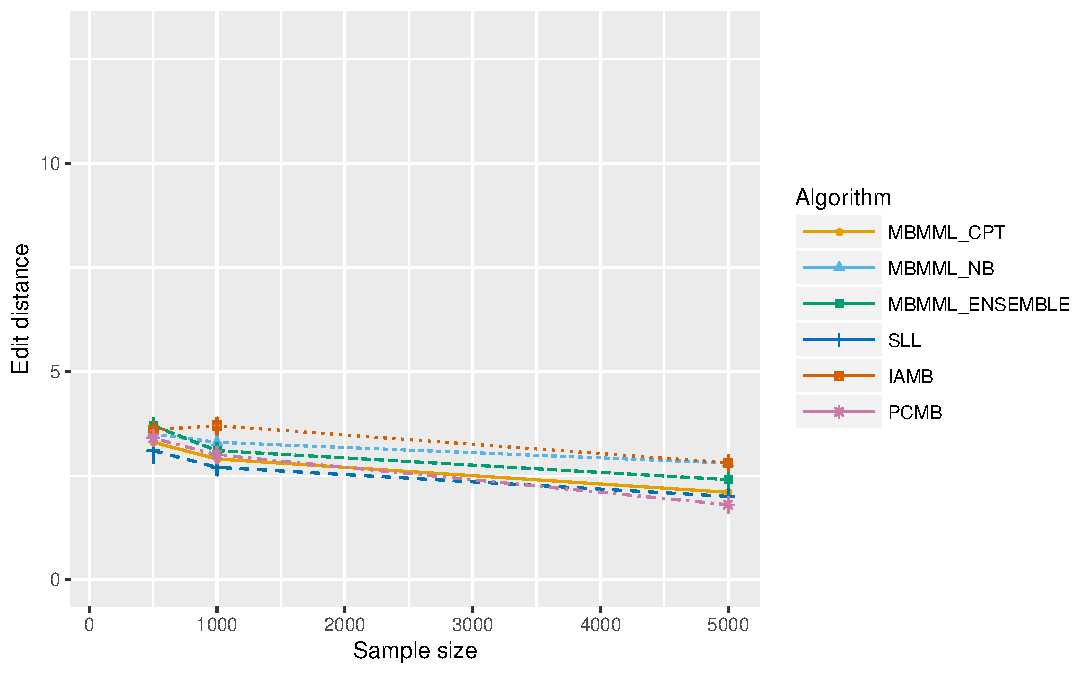
\includegraphics[scale=0.6]{figures/ed_vs_samplesize_insurance.pdf}
  \caption{Edit distance (with $95\%$ confidence intervals) v.s. sample size on INSURANCE network.}
\end{figure}

\begin{figure}[H]
  \centering
    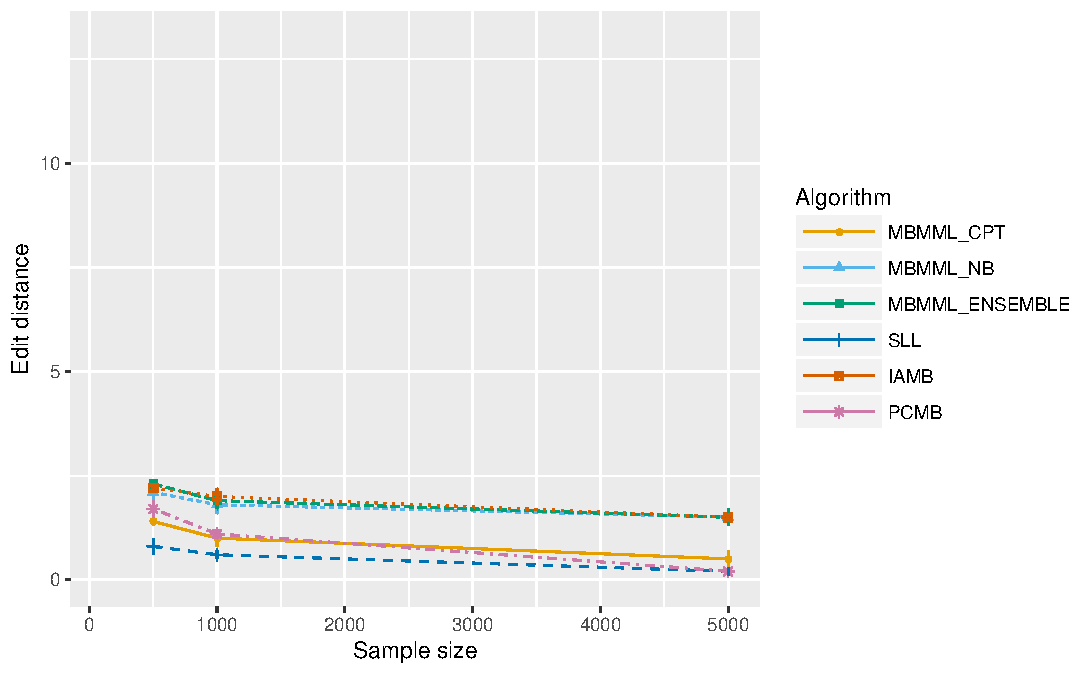
\includegraphics[scale=0.6]{figures/ed_vs_samplesize_alarm.pdf}
  \caption{Edit distance (with $95\%$ confidence intervals) v.s. sample size on ALARM network.}
\end{figure}

\begin{figure}[H]
  \centering
    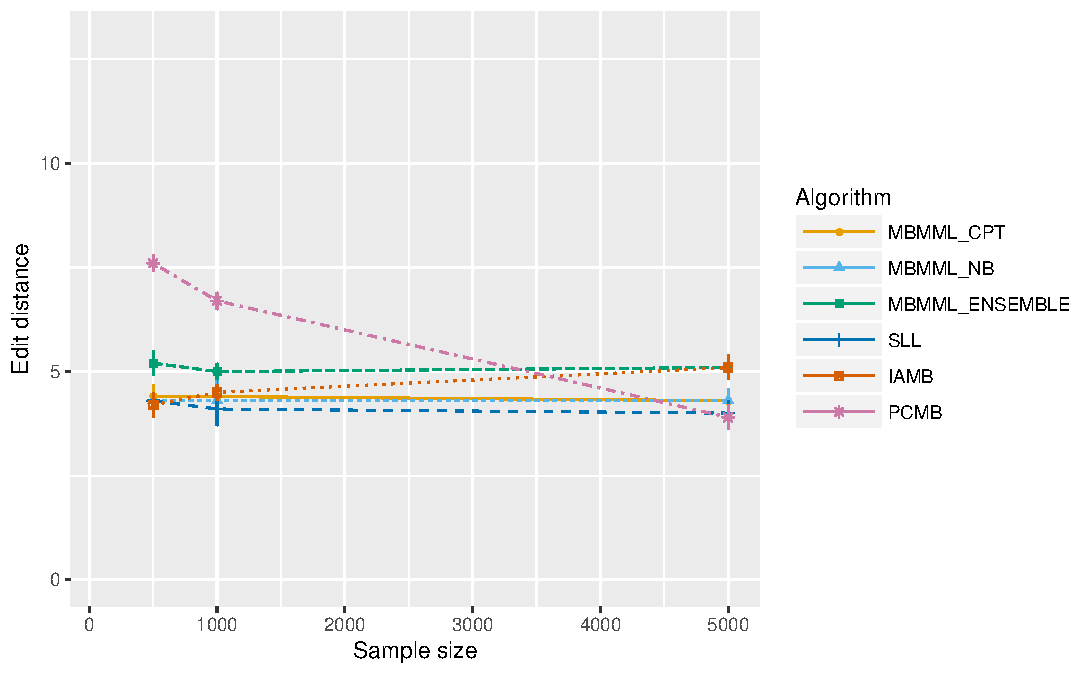
\includegraphics[scale=0.6]{figures/ed_vs_samplesize_hailfinder.pdf}
  \caption{Edit distance (with $95\%$ confidence intervals) v.s. sample size on HAILFINDER network.}
\end{figure}

\begin{figure}[H]
  \centering
    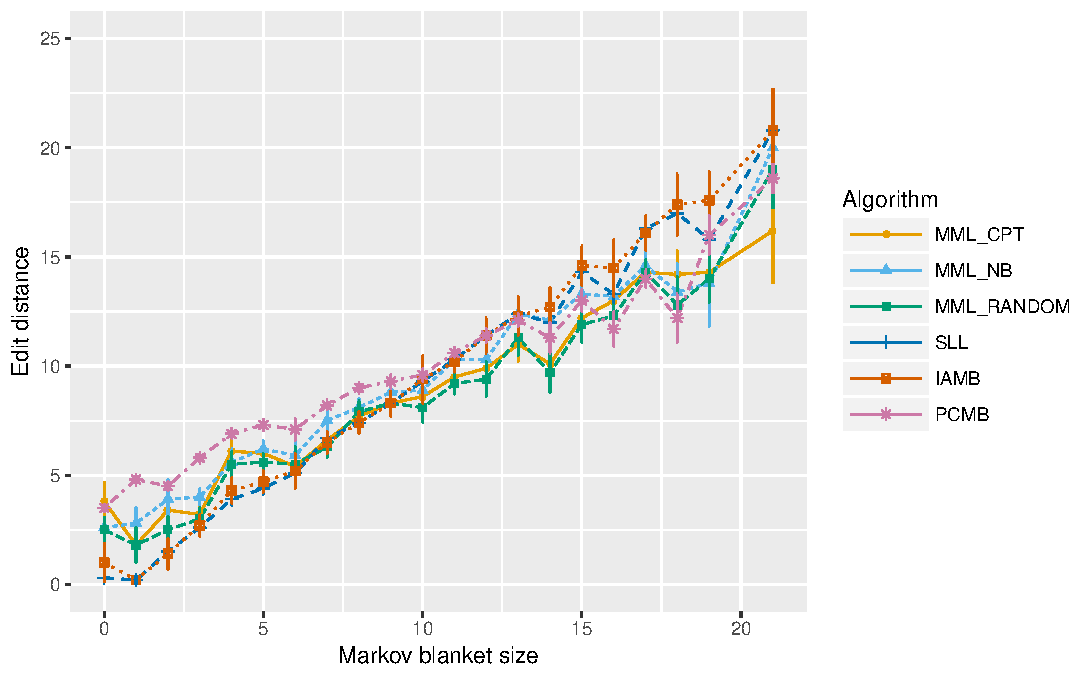
\includegraphics[scale=0.6]{figures/ed_vs_mbsize_30_5_4_1_100.pdf}
  \caption{Edit distance against Markov blanket size on 30-5-4-1 models with 100 samples.}
\end{figure} 

\begin{figure}[H]
  \centering
    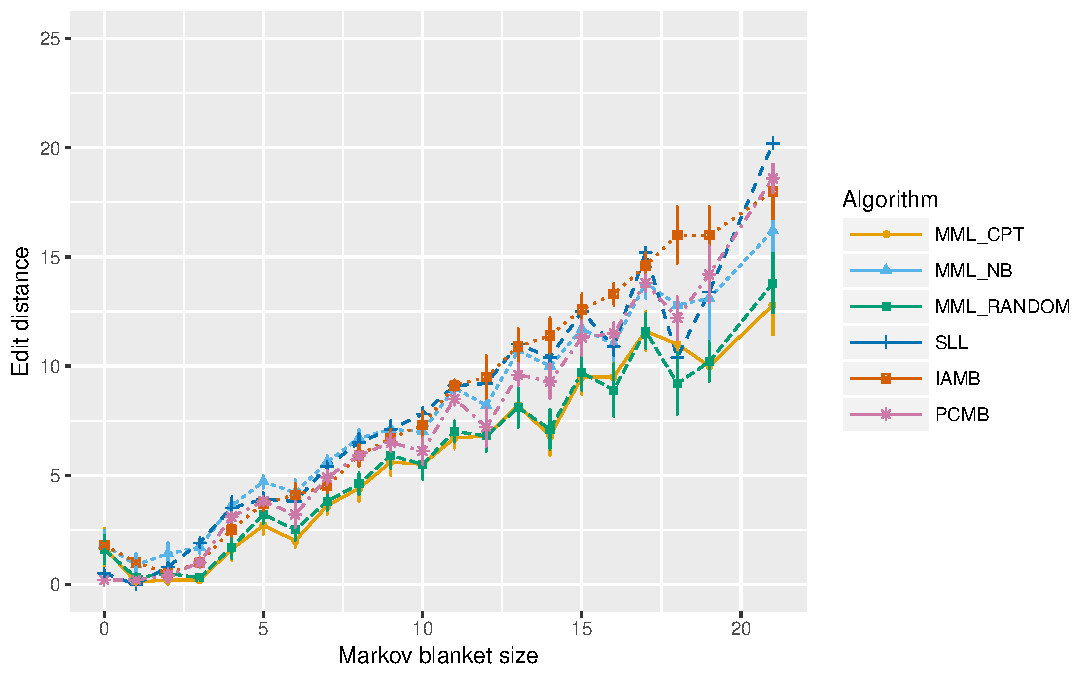
\includegraphics[scale=0.6]{figures/ed_vs_mbsize_30_5_4_1_500.pdf}
  \caption{Edit distance against Markov blanket size on 30-5-4-1 models with 500 samples.}
\end{figure}

\begin{figure}[H]
  \centering
    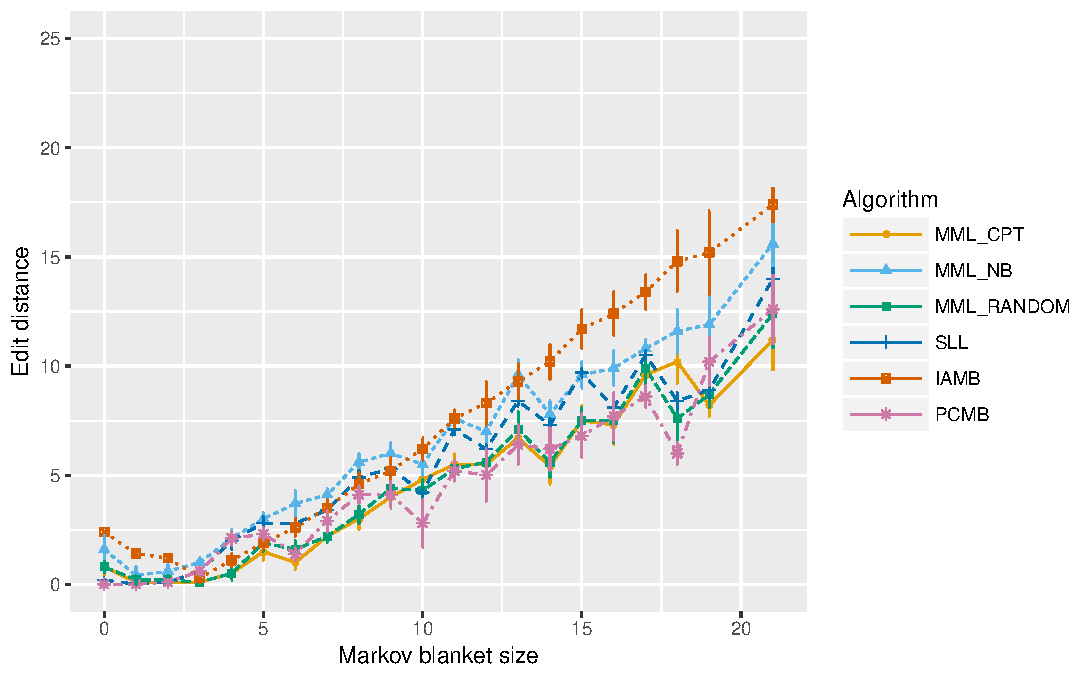
\includegraphics[scale=0.6]{figures/ed_vs_mbsize_30_5_4_1_2000.pdf}
  \caption{Edit distance against Markov blanket size on 30-5-4-1 models with 2000 samples.}
\end{figure} 

\begin{figure}[H]
  \centering
    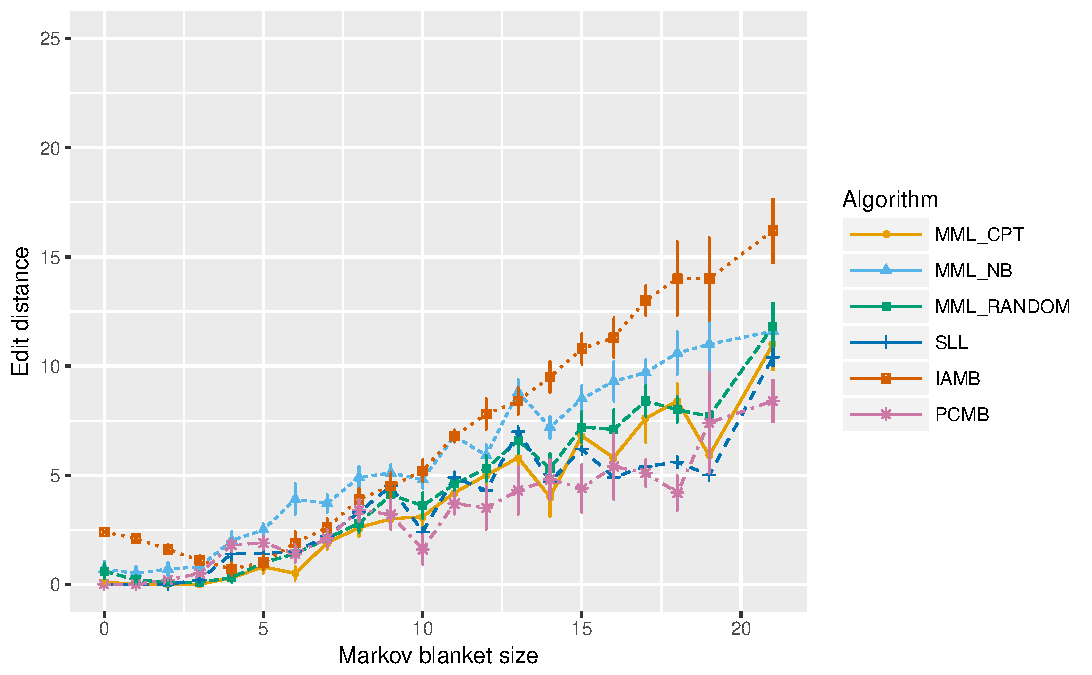
\includegraphics[scale=0.6]{figures/ed_vs_mbsize_30_5_4_1_5000.pdf}
  \caption{Edit distance against Markov blanket size on 30-5-4-1 models with 5000 samples.}
\end{figure} 

\begin{figure}[H]
  \centering
    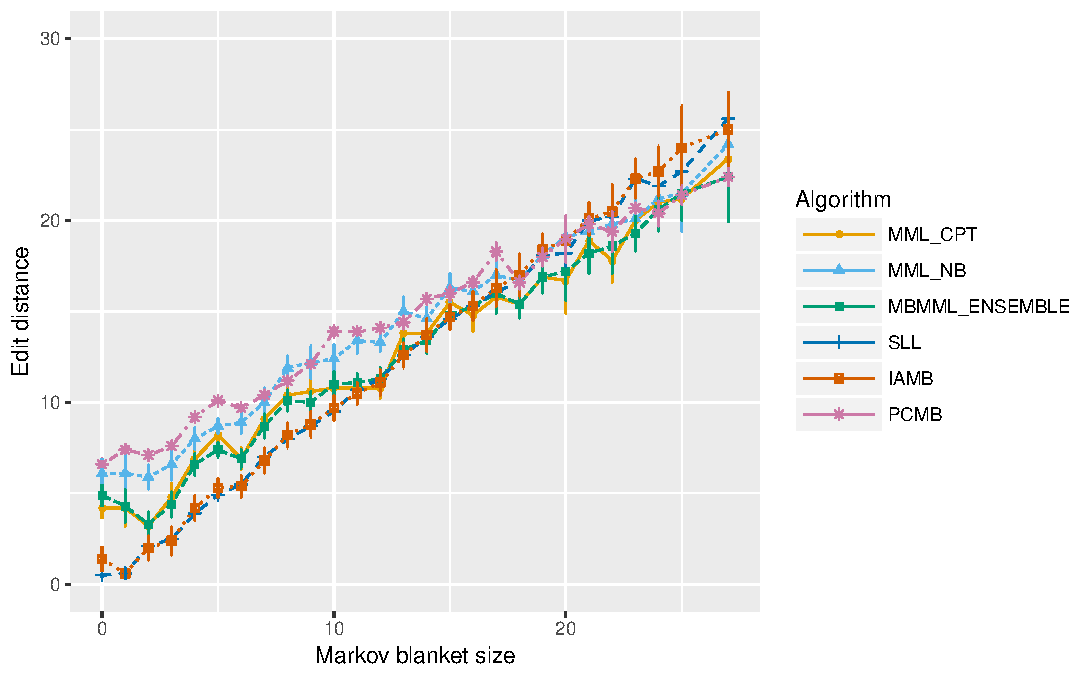
\includegraphics[scale=0.6]{figures/ed_vs_mbsize_50_5_4_1_100.pdf}
  \caption{Edit distance against Markov blanket size on 50-5-4-1 models with 100 samples.}
\end{figure} 

\begin{figure}[H]
  \centering
    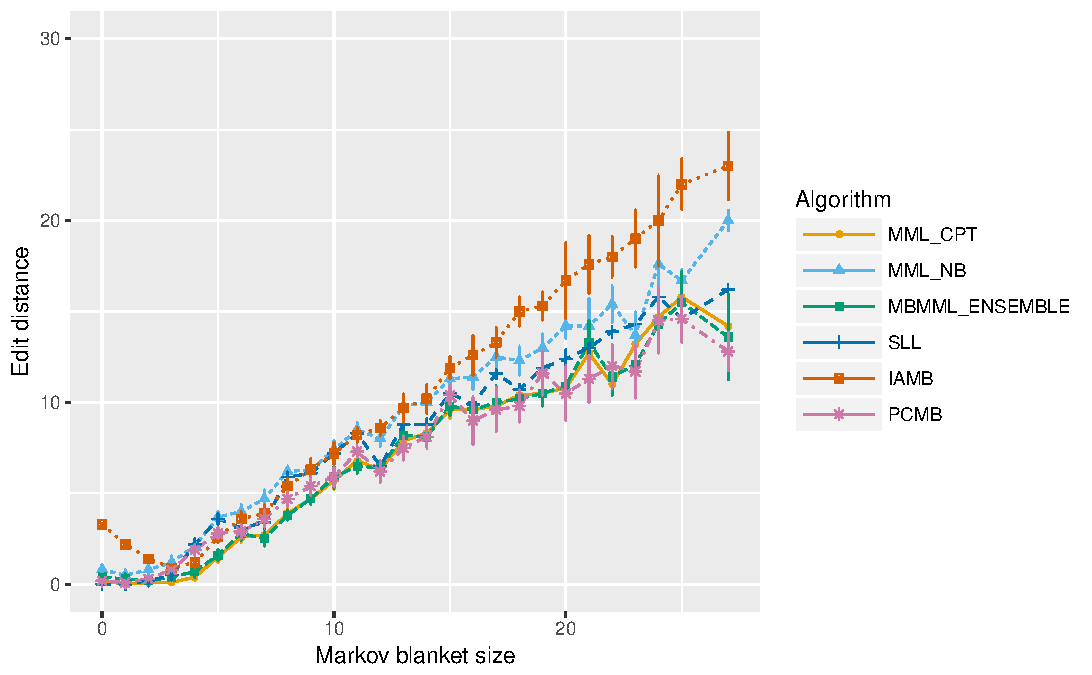
\includegraphics[scale=0.6]{figures/ed_vs_mbsize_50_5_4_1_2000.pdf}
  \caption{Edit distance against Markov blanket size on 50-5-4-1 models with 2000 samples.}
\end{figure} 

\newpage
\subsection{Notations}
\begin{table}[]
\centering
\caption{Notations}
\label{my-label}
\begin{tabular}{ll}
\hline
$G$ &  a directed acyclic graph\\
$X$ & a variable set \\ 
$E$ & an edge set \\
$P$ & a joint distribution \\
$<G, P>$ & a Bayesian network \\
$\mathcal{H}$ & a model class \\
$H$ & a hypothesis or model \\
$\theta$ &  a set model parameters\\
$\mathcal{D}$ & a set of datasets \\
$D$ & a dataset \\ 
$N$ & the number of observations in a dataset \\
$p(\cdot)$ & the probability of an event \\
$I(\cdot)$ & the information content or message length of an event\\
$|\cdot|$ & the cardinality of a set \\
$X_i$ & the $i^{th}$ variable in $X$ \\ 
$r_i$ & the number of states of a variable $X_i$ \\ 
$\Pi_i$ & a parents set of the variable $X_i$ \\ 
$r_{\Pi_i}$ & the total number of parents instantiations\\
$\vec{\alpha}$ & a vector of symmetric Dirichlet concentration parameters \\ 
$\alpha_i$ & the $i^{th}$ parameter in $\vec{\alpha}$ \\ 
$n_{ijk}$ & the count of $\Pi_i$ is in state $j$ and $X_i$ in state $k$, also known as sufficient statistics\\ 
$n_{ij}$ & the count of $\Pi_i$ in state $j$ \\ 
$T_i$ & a Markov blanket polytree of variable $X_i$ \\
$\mathcal{T}_i$ & a set of Markov blanket polytrees containing the same set of variables $\{X_i\}\cup MB_i$ \\ \hline
\end{tabular}
\end{table}

%\begin{acknowledgements}
%If you'd like to thank anyone, place your comments here
%and remove the percent signs.
%\end{acknowledgements}

% BibTeX users please use one of
%\bibliographystyle{spbasic}      % basic style, author-year citations
%\bibliographystyle{spmpsci}      % mathematics and physical sciences
%\bibliographystyle{spphys}       % APS-like style for physics
%\bibliography{}   % name your BibTeX data base
\newpage
\bibliographystyle{named}
\bibliography{/home/kl/Documents/causal_discovery_ref_list}

\end{document}
% end of file template.tex

